% \newcommand{\compacttitlespacing}{0} %disable when we need room for authors
\documentclass[sigconf,anonymous]{acmart}
\settopmatter{printacmref=false}
% defining the \BibTeX command - from Oren Patashnik's original BibTeX documentation.
\def\BibTeX{{\rm B\kern-.05em{\sc i\kern-.025em b}\kern-.08emT\kern-.1667em\lower.7ex\hbox{E}\kern-.125emX}}
    
\usepackage{nicefrac}
\usepackage{siunitx}
\usepackage{array,framed}
\usepackage{booktabs}
\usepackage{
  color,
  float,
  epsfig,
  wrapfig,
  graphics,
  graphicx,
  subcaption
}
% \usepackage[dvipsnames]{xcolor}
\usepackage{textcomp,amssymb}
\usepackage{setspace}
% \usepackage{amsfonts}
\usepackage{latexsym,fancyhdr,url}
\usepackage{enumerate}
\usepackage{algorithm2e}
\usepackage{algpseudocode}
\usepackage{graphics}
\usepackage{xparse} % argument parsing -- \edist
\usepackage{xspace}
\usepackage{multirow}
\usepackage{csvsimple}
\usepackage{balance}
\usepackage{booktabs}
\usepackage{array}
\usepackage{pifont}
\usepackage{graphicx}
% \usepackage{flushend}
% \usepackage{mathptmx,avant}

\newcommand{\cmark}{\ding{51}} % Checkmark
\newcommand{\xmark}{\ding{55}} % Crossmark

%%%% Tikz variables, pgfplot
\usepackage{
  tikz,
  pgfplots,
  pgfplotstable
}
\usepackage{hyperref}

\usetikzlibrary{
  shapes.geometric,
  arrows,
  external,
  pgfplots.groupplots,
  matrix
}

\pgfplotsset{compat=1.9}
% \tikzexternalize[prefix=images/]
% \tikzexternalenable

%\pagenumbering{arabic}
% \pagestyle{plain}

\usepackage{mathtools,}
\DeclarePairedDelimiter\abs{\lvert}{\rvert}
\DeclarePairedDelimiter\norm{\lVert}{\rVert}

% \setmathfont{Latin Modern Math}[version=lm]
\DeclareMathAlphabet{\mathcal}{OMS}{cmsy}{m}{n}
% \DeclareSymbolFont{operators}{T1}{cmr}{m}{n}
% \DeclareSymbolFont{letters}{OML}{cmm}{m}{it}
% \DeclareSymbolFont{symbols}{OMS}{cmsy}{m}{n}
% \DeclareSymbolFont{largesymbols}{OMX}{cmex}{m}{n}

% \usepackage{times}

% \setmathcal{Arial}

% TO deal with the weird flow of boxes
% \brokenpenalty=1000
% \clubpenalty=1000
% \widowpenalty=10
\DeclareGraphicsExtensions{%
    .png,.PNG,%
    .pdf,.PDF,%
    .jpg,.mps,.jpeg,.jbig2,.jb2,.JPG,.JPEG,.JBIG2,.JB2}

\usepackage{xparse}
\newcommand{\bnm}{\begin{newmath}}
\newcommand{\enm}{\end{newmath}}

\newcommand{\bea}{\begin{eqnarray*}}%
\newcommand{\eea}{\end{eqnarray*}}%

\newcommand{\bne}{\begin{newequation}}
\newcommand{\ene}{\end{newequation}}

\newcommand{\bal}{\begin{newalign}}
\newcommand{\eal}{\end{newalign}}

\newenvironment{newalign}{\begin{align}%
\setlength{\abovedisplayskip}{4pt}%
\setlength{\belowdisplayskip}{4pt}%
\setlength{\abovedisplayshortskip}{6pt}%
\setlength{\belowdisplayshortskip}{6pt} }{\end{align}}

\newenvironment{newmath}{\begin{displaymath}%
\setlength{\abovedisplayskip}{4pt}%
\setlength{\belowdisplayskip}{4pt}%
\setlength{\abovedisplayshortskip}{6pt}%
\setlength{\belowdisplayshortskip}{6pt} }{\end{displaymath}}

\newenvironment{neweqnarrays}{\begin{eqnarray*}%
\setlength{\abovedisplayskip}{-4pt}%
\setlength{\belowdisplayskip}{-4pt}%
\setlength{\abovedisplayshortskip}{-4pt}%
\setlength{\belowdisplayshortskip}{-4pt}%
\setlength{\jot}{-0.4in} }{\end{eqnarray*}}

\newenvironment{newequation}{\begin{equation}%
\setlength{\abovedisplayskip}{4pt}%
\setlength{\belowdisplayskip}{4pt}%
\setlength{\abovedisplayshortskip}{6pt}%
\setlength{\belowdisplayshortskip}{6pt} }{\end{equation}}


\newcounter{ctr}
\newcounter{savectr}
\newcounter{ectr}

\newenvironment{newitemize}{%
\begin{list}{\mbox{}\hspace{5pt}$\bullet$\hfill}{\labelwidth=15pt%
\labelsep=4pt \leftmargin=12pt \topsep=3pt%
\setlength{\listparindent}{\saveparindent}%
\setlength{\parsep}{\saveparskip}%
\setlength{\itemsep}{3pt} }}{\end{list}}


\newenvironment{newenum}{%
\begin{list}{{\rm (\arabic{ctr})}\hfill}{\usecounter{ctr} \labelwidth=17pt%
\labelsep=5pt \leftmargin=22pt \topsep=3pt%
\setlength{\listparindent}{\saveparindent}%
\setlength{\parsep}{\saveparskip}%
\setlength{\itemsep}{2pt} }}{\end{list}}

%%%%%%%%%%%%%%%%%%%%%%%%%%%%%%%%%%%%%%%%%%%%%%%%%%%%%%%%%%%%%%%%%%%%%%%%%%%%%%
%
% Figure and table macros
%

\newcounter{mytable}
\def\mytable{\begin{centering}\refstepcounter{mytable}}
\def\endmytable{\end{centering}}

\def\mytablecaption#1{\vspace{2mm}
  \centerline{Table \arabic{mytable}.~{#1}}
  \vspace{6mm}
  \addcontentsline{lot}{table}{\protect\numberline{\arabic{mytable}}~{#1}}
}


\newcounter{myfig}
\def\myfig{\begin{centering}\refstepcounter{myfig}}
\def\endmyfig{\end{centering}}

\def\myfigcaption#1{
             \vspace{2mm}
             \centerline{\textsf{Figure \arabic{myfig}.~{#1}}}
             \vspace{6mm}
             \addcontentsline{lof}{figure}{\protect\numberline{\arabic{myfig}}~{#1}}}


\newlength{\saveparindent}
\setlength{\saveparindent}{\parindent}
\newlength{\saveparskip}
\setlength{\saveparskip}{\parskip}

\newcommand{\decOracle}{\textbf{Dec}}

\newcommand{\negsmidge}{{\hspace{-0.1ex}}}
\newcommand{\cdotsm}{\negsmidge\negsmidge\negsmidge\cdot\negsmidge\negsmidge\negsmidge}

\def\suchthatt{\: :\:}
\newcommand{\E}{{\rm I\kern-.3em E}}
\newcommand{\Prob}[1]{{\Pr\left[\,{#1}\,\right]}}
\newcommand{\Probb}[2]{{\Pr}_{#1}\left[\,{#2}\,\right]}
\newcommand{\CondProb}[2]{{\Pr}\left[\: #1\:\left|\right.\:#2\:\right]}
\newcommand{\CondProbb}[2]{\Pr[#1|#2]}
\newcommand{\ProbExp}[2]{{\Pr}\left[\: #1\:\suchthatt\:#2\:\right]}
\newcommand{\Ex}[1]{{\textnormal{E}\left[\,{#1}\,\right]}}
\newcommand{\Exx}{{\textnormal{E}}}
\newcommand{\given}{\ensuremath{\,\big|\,}}


\newcommand{\true}{\mathsf{true}}
\newcommand{\false}{\mathsf{false}}
\def\negl{\mathsf{negl}}


\newcommand{\secref}[1]{\mbox{Section~\ref{#1}}}
\newcommand{\appref}[1]{\mbox{Appendix~\ref{#1}}}
\newcommand{\thref}[1]{\mbox{Theorem~\ref{#1}}}
\newcommand{\defref}[1]{\mbox{Definition~\ref{#1}}}
\newcommand{\corref}[1]{\mbox{Corollary~\ref{#1}}}
\newcommand{\lemref}[1]{\mbox{Lemma~\ref{#1}}}
\newcommand{\clref}[1]{\mbox{Claim~\ref{#1}}}
\newcommand{\propref}[1]{\mbox{Proposition~\ref{#1}}}
\newcommand{\factref}[1]{\mbox{Fact~\ref{#1}}}
\newcommand{\remref}[1]{\mbox{Remark~\ref{#1}}}
\newcommand{\figref}[1]{\mbox{Figure~\ref{#1}}}
\renewcommand{\algref}[1]{\mbox{Algorithm~\ref{#1}}}
% \newcommand{\eqref}[1]{\mbox{Equation~(\ref{#1})}}
% Have to use \renewcommand because exists already in amsmath
\renewcommand{\eqref}[1]{\mbox{Equation~(\ref{#1})}}
\newcommand{\consref}[1]{\mbox{Construction~\ref{#1}}}
\newcommand{\tabref}[1]{\mbox{Table~\ref{#1}}}

\newcommand{\get}{{\:{\leftarrow}\:}}
\newcommand{\gett}[1]{\:{\leftarrow}_{#1}\:}
\newcommand{\getsr}{{\:{\leftarrow{\hspace*{-3pt}\raisebox{.75pt}{$\scriptscriptstyle\$$}}}\:}}
\newcommand{\getm}{{\:\leftarrow_{\mdist}\:}}
\newcommand{\getd}{{\:\leftarrow_{\ddist}\:}}
%\newcommand{\getm}{{\:{\leftarrow{\hspace*{-3pt}\raisebox{.75pt}{$\scriptscriptstyle \mdist$}}}\:}}
\newcommand{\getk}{{\:\leftarrow_{\kdist}\:}}
%\newcommand{\getk}{{\:{\leftarrow{\hspace*{-3pt}\raisebox{.75pt}{$\scriptscriptstyle \kdist$}}}\:}}
\newcommand{\getp}{{\:\leftarrow_{p}\:}}



\newcommand{\gamesfontsize}{\small}
\newcommand{\fpage}[2]{\framebox{\begin{minipage}[t]{#1\textwidth}\setstretch{1.1}\gamesfontsize  #2 \end{minipage}}}
\newcommand{\mpage}[2]{\begin{minipage}[t]{#1\textwidth}\setstretch{1.1}\gamesfontsize  #2 \end{minipage}}

\newcommand{\hpages}[3]{\begin{tabular}{cc}\begin{minipage}[t]{#1\textwidth} #2 \end{minipage} & \begin{minipage}[t]{#1\textwidth} #3 \end{minipage}\end{tabular}}

\newcommand{\hpagess}[4]{
        \begin{tabular}[t]{c@{\hspace*{.5em}}c}
        \begin{minipage}[t]{#1\textwidth}\gamesfontsize #3 \end{minipage}
        &
        \begin{minipage}[t]{#2\textwidth}\gamesfontsize #4 \end{minipage}
        \end{tabular}
    }

\newcommand{\hpagesss}[6]{
        \begin{tabular}[t]{c@{\hspace*{.5em}}c@{\hspace*{.5em}}c@{\hspace*{.5em}}c}
        \begin{minipage}[t]{#1\textwidth}\gamesfontsize #4 \end{minipage}
        &
        \begin{minipage}[t]{#2\textwidth}\gamesfontsize #5 \end{minipage}
        &
        \begin{minipage}[t]{#3\textwidth}\gamesfontsize #6 \end{minipage}
        \end{tabular}
    }

\newcommand{\hpagessss}[8]{
        \begin{tabular}{c@{\hspace*{.5em}}c@{\hspace*{.5em}}c@{\hspace*{.5em}}c}
        \begin{minipage}[t]{#1\textwidth}\gamesfontsize #5 \end{minipage}
        &
        \begin{minipage}[t]{#2\textwidth}\gamesfontsize #6 \end{minipage}
        &
        \begin{minipage}[t]{#3\textwidth}\gamesfontsize #7 \end{minipage}
        &
        \begin{minipage}[t]{#4\textwidth}\gamesfontsize #8 \end{minipage}
        \end{tabular}
    }


\newcommand{\hfpages}[3]{\hfpagess{#1}{#1}{#2}{#3}}
\newcommand{\hfpagess}[4]{
        \begin{tabular}[t]{c@{\hspace*{.5em}}c}
        \framebox{\begin{minipage}[t]{#1\textwidth}\setstretch{1.1}\gamesfontsize #3 \end{minipage}}
        &
        \framebox{\begin{minipage}[t]{#2\textwidth}\setstretch{1.1}\gamesfontsize #4 \end{minipage}}
        \end{tabular}
    }
\newcommand{\hfpagesss}[6]{
        \begin{tabular}[t]{c@{\hspace*{.5em}}c@{\hspace*{.5em}}c}
        \framebox{\begin{minipage}[t]{#1\textwidth}\setstretch{1.1}\gamesfontsize #4 \end{minipage}}
        &
        \framebox{\begin{minipage}[t]{#2\textwidth}\setstretch{1.1}\gamesfontsize #5 \end{minipage}}
        &
        \framebox{\begin{minipage}[t]{#3\textwidth}\setstretch{1.1}\gamesfontsize #6 \end{minipage}}
        \end{tabular}
    }
\newcommand{\hfpagessss}[8]{
        \begin{tabular}[t]{c@{\hspace*{.5em}}c@{\hspace*{.5em}}c@{\hspace*{.5em}}c}
        \framebox{\begin{minipage}[t]{#1\textwidth}\setstretch{1.1}\gamesfontsize #5 \end{minipage}}
        &
        \framebox{\begin{minipage}[t]{#2\textwidth}\setstretch{1.1}\gamesfontsize #6 \end{minipage}}
        &
        \framebox{\begin{minipage}[t]{#3\textwidth}\setstretch{1.1}\gamesfontsize #7 \end{minipage}}
        &
        \framebox{\begin{minipage}[t]{#4\textwidth}\setstretch{1.1}\gamesfontsize #8 \end{minipage}}
        \end{tabular}
    }

\newcommand{\vecw}{\mathbf{w}}
\newcommand{\R}{\mathbb{R}}
\newcommand{\N}{\mathbb{N}}
\newcommand{\Z}{\mathbb{Z}}
\newcommand{\load}{L}
\newcommand{\coll}{\mathsf{Coll}}
\newcommand{\nocoll}{\overline{\mathsf{Coll}}}


\newcommand{\Img}{\textsf{Img}}

%%%%%%%%%%%%%%%%%%%%%%%%%%%%%%%%%%%%%%%%%%%%%%%%%%%%%%%%%%%%%%%%%%%%%%%%%%%%%%%%
%%%% Fonts and symbols
%%%%%%%%%%%%%%%%%%%%%%%%%%%%%%%%%%%%%%%%%%%%%%%%%%%%%%%%%%%%%%%%%%%%%%%%%%%%%%%%
\newcommand\funcfont{\textsf}
\newcommand\variablefont{\texttt}

%%%%%%%%%%%%%%%%%%%%%%%%%%%%%%%%%%%%%%%%%%%%%%%%%%%%%%%%%%%%%%%%%%%%%%%%%%%%%%%%
%%%%%%%%%%%%%%%%%%%%%%%%%%%%%%%% NEW COMMANDS %%%%%%%%%%%%%%%%%%%%%%%%%%%%%%%%%%
%%%%%%%%%%%%%%%%%%%%%%%%%%%%%%%%%%%%%%%%%%%%%%%%%%%%%%%%%%%%%%%%%%%%%%%%%%%%%%%%

\def \Perm {\funcfont{Perm}}
\def \calC {{\mathcal{C}}}
\def \calU {{\mathcal{U}}}
\renewcommand{\u}{\ensuremath{u}}
\newcommand{\unew}{\ensuremath{\tilde{u}}}

\newcommand{\calN}{\mathcal{N}}
\def \sspace {{\mathcal{S}}}
\def \strings {{\mathcal{S}}}
\def \slen {{s}}
\def \kspace {{\mathcal{K}}}
\def \kspacesize {{m}}
\def \mspacesize {{n}}
\def \kdict {D}
\def \dictsize {d}
\newcommand{\kdist}{p_k}
\newcommand{\mdist}{\ensuremath{{W}}}
\newcommand{\alldist}{\rho}
\newcommand{\pwdist}{\transgen}
\newcommand{\ddist}{\rho_{dec}}
\newcommand{\PWset}{{\mathcal{P}}}  % TODO: fix, same as \pwdist
\newcommand{\PWsetvec}{\vec{\mathcal{P}}}
\newcommand{\PWvec}{\vec{P}}
\newcommand{\domvec}{\vec{D}}
\newcommand{\humanornot}{\vec{h}}
\newcommand{\dom}{\textsf{dom}}
%\def \kdist {{\kappa}}
%\def \mdist {{\mu}}
%\def \ddist {{\delta}}
\def \pspace {{\mathcal{P}}}
\def \mpspace {{\mathcal{MP}}}
\def \cspace {{\mathcal{C}}}
\def \key {\kappa}
\def \msg {M}
\def \seed {S}
\def \ctxt {C}
\def \ctxtpart {C_2}
\newcommand{\genprime}{{\textsf{GenPrime}}}
\newcommand{\isprime}{{\textsf{IsPrime}}}
\newcommand{\LeastLesserPrime}{{\textsf{PrevPrime}}}
\newcommand{\pwset}{\mathcal{S}}
\newcommand{\DTE}{{\textsf{DTE}}}
\newcommand{\encode}{{\textsf{encode}}}
\newcommand{\decode}{{\textsf{decode}}}

\newcommand{\DTEsingle}{{\textsf{1PW-DTE}}}
\newcommand{\encodesingle}{{\textsf{1PW-encode}}}
\newcommand{\decodesingle}{{\textsf{1PW-decode}}}

\newcommand{\DTErss}{{\textsf{RSS-DTE}}}
\newcommand{\encoderss}{{\textsf{RSS-encode}}}
\newcommand{\decoderss}{{\textsf{RSS-decode}}}

\newcommand{\DTEindep}{{\textsf{MPW-DTE}}}
\newcommand{\encodeindep}{{\textsf{MPW-encode}}}
\newcommand{\decodeindep}{{\textsf{MPW-decode}}}


\newcommand{\DTEsub}{{\textsf{SG-DTE}}}
\newcommand{\encodesub}{{\textsf{SG-encode}}}
\newcommand{\decodesub}{{\textsf{SG-decode}}}
\newcommand{\decodekamf}{{\textsf{KAMF-decode}}}
\newcommand{\DTEis}{{\textsf{IS-DTE}}}
\newcommand{\encodeis}{{\textsf{is-encode}}}
\newcommand{\decodeis}{{\textsf{is-decode}}}
\newcommand{\DTErej}{{\textsf{REJ-DTE}}}
\newcommand{\encoderej}{{\textsf{rej-encode}}}
\newcommand{\decoderej}{{\textsf{rej-decode}}}
\newcommand{\DTErsarej}{{\textsf{RSA-REJ-DTE}}}
\newcommand{\encodeRSAREJ}{{\textsf{rsa-rej-encode}}}
\newcommand{\decodeRSAREJ}{{\textsf{rsa-rej-decode}}}
\newcommand{\DTErsainc}{{\textsf{RSA-INC-DTE}}}
\newcommand{\encodeRSAINC}{{\textsf{rsa-inc-encode}}}
\newcommand{\decodeRSAINC}{{\textsf{rsa-inc-decode}}}
\newcommand{\DTEunf}{{\textsf{UNF-DTE}}}
\newcommand{\DTEnunf}{{\textsf{NUNF-DTE}}}


%\newcommand{\encodeis}{{\textsf{encode}_{\textrm{is}}}}
%\newcommand{\decodeis}{{\textsf{decode}_{\textrm{is}}}}
\newcommand{\rep}{\textsf{rep}}
\newcommand{\isErr}{\epsilon_{\textnormal{is}}}
\newcommand{\incErr}{\epsilon_{\textnormal{inc}}}
\def \enc {{\textsf{E}}}
\def \dec {{\textsf{D}}}
\def \SEscheme {{\textsf{SE}}}
\def \HEscheme {{\textsf{HE}}}
\def \CTR {{\textsf{CTR}}}
\def \encHE {{\textsf{HEnc}}}
\def \HIDE {{\textsf{HiaL}}}
\def \encHIDE {{\textsf{HEnc}}}
\def \decHIDE {{\textsf{HDec}}}
\def \decHE {{\textsf{HDec}}}
\def \encHEt {{\textsf{HEnc2}}}
\def \decHEt {{\textsf{HDec2}}}

\newcommand{\myind}{\hspace*{1em}}
\newcommand{\thh}{^{\textit{th}}} % th
\newcommand{\concat}{\,\|\,}
\newcommand{\dotdot}{..}
\newcommand{\emptystr}{\varepsilon}

\newcommand{\round}{\textsf{round}}

\newcommand{\alphabar}{\overline{\alpha}}
\newcommand{\numbinsbar}{\overline{b}}
\newcommand{\numballs}{a}
\newcommand{\numbins}{b}

%\def \encHE {{\sf{enc}^{HE}}}
%\def \decHE {{\sf{dec}^{HE}}}
%\def \encHEt {{\sf{enc}^{HE2}}}
%\def \decHEt {{\sf{dec}^{HE2}}}
\def \idealHE {{\mathcal{HE}}}
\def \IEnc {{\mathbf{\rho}}}
\def \IDec {{\mathbf{\rho^{-1}}}}
\def \OEnc {{\mathbf{Enc}}}
\def \ODec {{\mathbf{Dec}}}
\newcommand{\SimuProc}{\mathbf{Sim}}
\newcommand{\ROProc}{\mathbf{RO}}
\newcommand{\PrimProc}{\mathbf{Prim}}
\def \stm {g}
\def \istm {\hat{g}}
\def \kts {{f}}
\def \lex {{\sf lex}}
\def \part {part}
\def \kd {{\sf{kd}}}
\def \msgdist {{d}}
\def \keydist {{r}}
\def \ind {{\sf{index}}}
\def \kprf {z}
\def \adv {{\mathcal A}}
\def \pwds {u}
\newcommand{\mpw}{mpw}
\newcommand{\pw}{w}
\newcommand{\pwvec}{\vec{\pw}}
\newcommand{\vecx}{\vec{x}}
\def \tokens {v}
\def \calP{{\mathcal{P}}}
\def \template{{\mathcal{T}}}
\def \vaultset{{\mathcal{V}}}
\def \ext {{\sf ext}}
\def \offset {\delta}
\def \maxweight {\epsilon}
\def \advo {{\mathcal{A}}^{*}}

\newcommand{\Chall}{\textsf{Ch}}
\newcommand{\Test}{\textnormal{\textsf{Test}}}
\newcommand{\RoR}{\textsf{RoR}}
\newcommand{\MI}{\textnormal{MI}}
\providecommand{\MR}{\textnormal{MR}}
\newcommand{\MRCCA}{\textnormal{MR-CCA}}
\newcommand{\SAMP}{\textnormal{SAMP}}
\newcommand{\DTEgame}{\textnormal{SAMP}}
\newcommand{\KR}{\textnormal{KR}}
\newcommand{\advA}{{\mathcal{A}}}
\newcommand{\advR}{{\mathcal{R}}}
\newcommand{\advB}{{\mathcal{B}}} % 
\newcommand{\advC}{{\mathcal{C}}} % C
\newcommand{\advD}{{\mathcal{D}}} % D
\newcommand{\advE}{{\mathcal{E}}}
\newcommand{\advF}{{\mathcal{F}}}
\newcommand{\advG}{{\mathcal{G}}}
\newcommand{\advI}{{\mathcal{I}}}
\newcommand{\nextval}{\;;\;}
\newcommand{\TabC}{\texttt{C}}
\newcommand{\TabR}{\texttt{R}}
\newcommand{\Hash}{H}
\newcommand{\Cipher}{\pi}
\newcommand{\CipherInv}{\pi^{-1}}
\newcommand{\simu}{{\mathcal S}}
\newcommand{\prim}{P}
\newcommand{\maxguess}{\gamma}


\newcommand{\bigO}{\mathcal{O}}
\newcommand{\calG}{{\mathcal{G}}}

\def\sqed{{\hspace{5pt}\rule[-1pt]{3pt}{9pt}}}
\def\qedsym{\hspace{2pt}\rule[-1pt]{3pt}{9pt}}

\newcommand{\Colon}{{\::\;}}
\newcommand{\good}{\textsf{Good}}

\newcommand\Tvsp{\rule{0pt}{2.6ex}}
\newcommand\Bvsp{\rule[-1.2ex]{0pt}{0pt}}
\newcommand{\TabPad}{\hspace*{5pt}}
\newcommand\TabSep{@{\hspace{5pt}}|@{\hspace{5pt}}}
\newcommand\TabSepLeft{|@{\hspace{5pt}}}
\newcommand\TabSepRight{@{\hspace{5pt}}|}


\DeclareMathOperator*{\argmin}{argmin}
\DeclareMathOperator*{\argmax}{argmax}
\newcommand{\comma}{\textnormal{,}}

\renewcommand{\paragraph}[1]{\vspace*{6pt}\noindent\textbf{#1}\;}

\newcommand{\weirvault}{\textsf{Pastebin}\xspace}
\newcommand{\ndssvault}{\textsf{DBCBW}\xspace}




\newcommand{\reminder}[1]{ [[[ \marginpar{\mbox{$<==$}} #1 ]]] }

%
% New theorem types: (Already in CCS template)
%
\newtheorem{observation}{Observation}
%\newtheorem{definition}{Definition}
\newtheorem{claim}{Claim}
\newtheorem{assumption}{Assumption}
\newtheorem{fact}{Fact}
% \newtheorem{theorem}{Theorem}[section]
% \newtheorem{lemma}{Lemma}[section]
% \newtheorem{corollary}{Corollary}[section]
% \newtheorem{proposition}{Proposition}
% \newtheorem{example}{Example}

%
% Definitions:
%
\def \blackslug{\hbox{\hskip 1pt \vrule width 4pt height 8pt
    depth 1.5pt \hskip 1pt}}
\def \qed{\quad\blackslug\lower 8.5pt\null\par}
% In-line QED, for ending a proof with a $$ formula
% In-line QED, for ending a proof with a $$ formula
\def \inQED{\quad\quad\blackslug}
\def \Qed{\QED}
\def \QUAD{$\Box$}
\def \Proof{\par\noindent{\bf Proof:~}}
\def \proof{\Proof}
\def \poly {\mbox{$\mathsf{poly}$}}
\def \binary {\mbox{$\mathsf{binary}$}}
\def \ones {\mbox{$\mathsf{ones}$}}
\def \rank {\mbox{$\mathsf{rank}$}}
\def \bits {\mbox{$\mathsf{bits}$}}
\def \factorial {\mbox{$\mathsf{factorial}$}}
\def \fr {\mbox{$\mathsf{fr}$}}
\def \pr {\mbox{$\mathsf{pr}$}}
\def \zon {\{0,1\}^n}
\def \zo  {\{0,1\}}
\def \zok {\{0,1\}^k}
\def \mo {s}


\def\utilcnt{\ensuremath{\mu_{\mathrm{cnt}}}}
\def\utiltime{\ensuremath{\mu_{\mathrm{time}}}}
\def\ex{\ensuremath{{\mathrm{ex}}}}
\def\rlx{\ensuremath{{\mathrm{rlx}}}}
\def\tp{\textsf{TP}}
\def\cp{\textnormal{\textsf{CP}}\xspace}
\def\edistcutoff{\edist}
\def\entcutoff{\ensuremath{m}}
\def\relentcutoff{{\sigma}}
\def\mutt{\mu_{\mathrm{tt}}}

\newcommand{\Hdot}{H(\mbox{ } \cdot \mbox{ }  , \mbox{ } \del)}


\newcounter{mynote}[section]
\newcommand{\notecolor}{blue}
\newcommand{\thenote}{\thesection.\arabic{mynote}}
\newcommand{\tnote}[1]{\refstepcounter{mynote}{\bf \textcolor{\notecolor}{$\ll$TomR~\thenote: {\sf #1}$\gg$}}}

\newcommand{\fixme}[1]{{\textcolor{red}{[FIXME: #1]}}}
\newcommand{\todo}[1]{{\textcolor{red}{[TODO: #1]}}}


\newcommand\ignore[1]{}


\newcommand\simplescheme{simple}


\newcommand{\KDF}{\mathsf{KDF}}
\newcommand{\salt}{\mathsf{sa}}
\newcommand{\PRF}{F}
\newcommand{\subgram}{\mathsf{SG}}
\newcommand{\popdomains}{\mathcal{D}}

\newcommand{\retrieve}{\textsf{Sync}}
\newcommand{\update}{\textsf{Insert}}

\newcommand{\dictW}{\textbf{D1}\xspace}
\newcommand{\dictF}{\textbf{D2}\xspace}

\newcommand{\str}{\text{str}}
\newcommand{\calS}{{\mathcal S}}

% \newcommand{\new}[1]{\textcolor{red}{\sf #1}}
\newcommand{\new}[1]{#1}


%% ------------------------- Rahul -----------------------
\newcounter{rcnote}[section]
\newcommand{\rcthenote}{\thesection.\arabic{rcnote}}
\newcommand{\rcnote}[1]{\refstepcounter{rcnote}{\bf \textcolor{magenta}{$\ll$RC~\rcthenote: {\sf #1}$\gg$}}}

\newcounter{mrnote}[section]
\newcommand{\mrthenote}{\thesection.\arabic{mrnote}}
\newcommand{\mrnote}[1]{\refstepcounter{mrnote}{\bf \textcolor{green}{$\ll$MR~\mrthenote: {\sf #1}$\gg$}}}

\newcounter{fknote}[section]
\newcommand{\fkthenote}{\thesection.\arabic{fknote}}
\newcommand{\fknote}[1]{\refstepcounter{fknote}{\bf \textcolor{blue}{$\ll$FK~\fkthenote: {\sf #1}$\gg$}}}

\newcounter{anote}[section]
\newcommand{\ajthenote}{\thesection.\arabic{anote}}
\newcommand{\anote}[1]{\refstepcounter{anote}{\bf \textcolor{cyan}{$\ll$AJ~\ajthenote: {\sf #1}$\gg$}}}



\newcommand{\mytab}{\hspace*{.4cm}}
\def\half{{1\over 2}}
\newcommand{\NT}[1]{\texttt{#1}}
\DeclareMathSymbol{\mlq}{\mathord}{operators}{``}
\DeclareMathSymbol{\mrq}{\mathord}{operators}{`'}
\newcommand{\calO}{{\mathcal O}}
\newcommand{\calA}{{\mathcal A}}
\newcommand{\kamfplus}{Kamouflage\textbf{+}\xspace}
% \newcommand{\genfrom}[1]{\;{\stackrel{\,#1}{\leftarrow}}\;}
\newcommand{\genfrom}[1]{{\:{\leftarrow{\hspace*{-3pt}\raisebox{.75pt}{$\scriptscriptstyle#1$}}}\:}}
%\newcommand{\genfrom}[1]{\;\leftarrow{\tiny \$} #1\;}
\newcommand{\twopartdef}[4]
{
  \left\{
    \begin{array}{ll}
      #1 & \mbox{if } #2 \\[4pt]
      #3 & #4
      \end{array}
      \right.
}
\newcommand{\threepartdef}[6]
{
  \left\{
    \begin{array}{lll}
      #1 & \mbox{if } #2 \\
      #3 & \mbox{if } #4 \\
      #5 & \mbox{if } #6
      \end{array}
      \right.
}

\newcommand{\gt}[1]{\gamma_{#1,\maxdist}}
\newcommand{\gmt}[2]{\gamma_{#1,#2}}
\def\nh{\ensuremath{N}}
\def\ball{\ensuremath{B}}
\def\anh{\ensuremath{\tilde{N}_k}}
% \newcommand{\nh}[2]{{N_{#1}(#2)}}

\newcommand{\ballsizet}[1]{{\beta_{#1,\maxdist}}}
\newcommand{\ballsize}[2]{{\beta_{#1,#2}}}
\newcommand{\rh}[2]{{\bf R}_{#1, #2}}
\newcommand{\rhf}[2]{R_{f, \gamma}}
\newcommand{\realm}{{m}}
% \newcommand{\inputm}{{\tilde{m}}}
\newcommand{\lmid}{\ell_{\realm, m'}}
\newcommand{\cipherlength}{n}
\renewcommand{\SS}{\textsf{SS}}
\newcommand{\Rec}{\textsf{Rec}\xspace}
\newcommand{\rec}{\textsf{rec}\xspace}
\newcommand{\Rep}{\textsf{Rep}\xspace}
\newcommand{\Gen}{\textsf{Gen}}
\newcommand{\dis}{\textsf{dis}}

\def\chk{\textnormal{\textsf{Chk}}\xspace}
\def\reg{\textnormal{\textsf{Reg}}\xspace}
\def\exchk{\textnormal{\textsf{ExChk}}\xspace}
\def\adpchk{\textnormal{\textsf{AdpChk}}\xspace}
\def\RKROR{\textnormal{MKROR}\xspace}
\def\SRKROR{\textnormal{SKROR}\xspace}
\def\ROR{\textnormal{ROR}\xspace}
\def\ROBUST{\textnormal{ROB}\xspace}
\def\OFFDIST{\textnormal{OFFDIST}\xspace}
\def\POFFDIST{\overline{\textnormal{OFFDIST}}\xspace}
\def\OFFGUESS{\textnormal{OFFGUESS}\xspace}
\def\ONGUESS{\overline{\textnormal{ONGUESS}}\xspace}
\def\ONATTACK{\textnormal{ONATTACK}\xspace}
\def\adp{\ensuremath{\Pi\xspace}}
\def\Check{\textnormal{\textsf{Checker}}}
\def\CheckPtxt{\textnormal{\textsf{PChecker}}}
\def\trans{\textnormal{\ensuremath{T}}}
\def\transgen{\textnormal{\ensuremath{\mathcal{T}}}}
\def\pke{\ensuremath{\mathcal{E}}}
\def\pkenc{\ensuremath{\pke^{\mathrm{enc}}}}
\def\pkdec{\ensuremath{\pke^{\mathrm{dec}}}}
\def\sH{\ensuremath\mathrm{H}^s}
\def\H{\ensuremath{\mathsf{H}}\xspace}
\def\T{\ensuremath{\mathsf{T}}\xspace}
\def\W{\ensuremath{\mathsf{W}}\xspace}
\def\F{\ensuremath{\mathsf{F}}\xspace}
\def\ret{\ensuremath{\mathrm{return}}\xspace}
\def\cs{\ensuremath{t}} % Cache Size
\def\waitlen{\ensuremath{\omega}\xspace} %waitlist size
\newcommand{\M}{{\mathcal{M}}}
\newcommand{\ent}{{\bf H}}
\newcommand{\Hfuzzy}{{\mathrm{H}}^{\rm fuzz}}
\newcommand{\Hminfuzzy}{{\mathrm{H}}^{{\rm{fuzz}}}_{t,\infty}}
\newcommand{\Hpfuzzy}{{\mathrm{H}}^{{\rm{pfuzz}}}}
\newcommand{\Hinf}{{\bf H}^{{\rm \min}}_{\infty}}
\newcommand{\Hminpfuzzy}{{\bf H}^{{\rm pfuzz}}_{t,\infty}}


\def\sa{{\sf sa}}
\def\err{{\varepsilon}}%^{(e)}}}
\newcommand{\dist}{\mathcmd{p}}
\newcommand{\distest}{\hat{\mathcmd{p}}}
\newcommand{\distvec}{\mathbf{\dist}}
\newcommand{\distvecest}{\hat{\mathbf{p}}}
\newcommand{\w}{{w}}
\newcommand{\wnew}{\tilde{w}}
\newcommand{\m}{{w}}
\newcommand{\mnew}{{\tilde{m}}}
\newcommand{\mspacevec}{\mathcmd{\mathbf{W}}}
\newcommand{\mvec}{\mathcmd{\mathbf{\m}}}
\newcommand{\mvecss}[1]{\mvec_1\ldots\mvec_{#1}}
\renewcommand{\mspace}{\mathcmd{W}}
\newcommand{\mspacebot}{{\mspace}_\bot}

\newcommand{\similar}{\mathrm{sim}}
\newcommand{\similarvec}{\mathrm{\mathbf{sim}}}

\def \mvecnew{{\tilde{\mvec}}}
\newcommand{\mvecnewss}[1]{\mvecnew_1\ldots\mvecnew_{#1}}

\DeclareDocumentCommand{\edist}{o o}{
  \ensuremath{
    \IfNoValueTF{#1}{{d}}{{\sf d}(#1,#2)}
  }
}

\newcommand{\utilinc}{\mu}
\newcommand{\secloss}{\Delta}
\newcommand{\seclossg}{\Delta^\textnormal{greedy}}
\newcommand{\seclosso}{\Delta}
%\newcommand{\maxlambda}{\lambda^*}
%\newcommand{\maxfuzzlambda}{\tilde{\lambda}^*}
\newcommand{\fuzzlambda}{\lambda^\textnormal{fuzzy}}
\newcommand{\greedylambda}{\lambda^\textnormal{greedy}}
\newcommand{\greedylambdaon}{\tilde{\lambda}^\mathrm{on}}
\newcommand{\greedylambdaoff}{\tilde{\lambda}^\mathrm{off}}
\newcommand{\seclosson}{\secloss^\mathrm{on}}
\newcommand{\seclossoff}{\secloss^\mathrm{off}}
\def \edit {\ensuremath{e}}
\newcommand\error{e}
\newcommand\tab[1][1cm]{\hspace*{#1}}

\newcommand{\mathcmd}[1]{\ensuremath{#1}\xspace} % to use a command both in math mode and non-math mode
\newcommand{\minentropy}[1]{\ensuremath{\operatorname{H_\infty}\olrk{#1}}}
\newcommand{\fuzzyminentropy}[1]{\ensuremath{\operatorname{H^{fuzz}_{\maxdist, \infty}}\olrk{#1}}}
\providecommand{\condminentropy}[2]{\ensuremath{\operatorname{\tilde{H}_\infty}\olrk{#1|#2}}}
\newcommand{\s}{\mathcmd{s}}
\newcommand{\typo}{\mathcmd{\tilde{\m}}}
\newcommand{\typoj}[1]{\ensuremath{(\typo_{#1}, j_{#1})}}
\newcommand\typojprime[1]{{(\typo_{#1}, j'_{#1})}}
\renewcommand\contrib[2]{\mathsf{cont}\left[{#1}/{#2}\right]}
\def\typovec{\ensuremath{\{\typo_i\}_{i=1}}}
\def\opttypovec{\ensuremath{\{\typo^*_i\}_{i=1}}}
\def\slotguess{\textsf{SlotGuess}}
\def\typodist{\ensuremath{\tau_\pw}}
\def\cachedtypodist{\ensuremath{{\tilde{\tau}}_{\pw}}}
\def\typodistest{\ensuremath{{\hat{\tau}}_{\pw}}}
\def\incache{T_\pw}
\newcommand{\fuzzylambda}{\ensuremath{\lambda^{\mathrm{fuzzy}}}}
%\newcommand{\errorprob}[2]{\mathcmd{\tau_{#1}({#2})}}
\newcommand{\errordist}{\mathcmd{\tau}}
\newcommand{\famdist}{\mathcmd{\mathcal{W}}}
\def\guessw{\ensuremath{W}}
\newcommand{\precdist}{W}
\newcommand{\entdef}{Z}
\newcommand{\PW}{\mathcmd{\mathcal{W}}}
\newcommand{\cachedom}{\mathcmd{\mathcal{S}}}
\newcommand{\supp}{\mbox{supp}}
\newcommand{\olrk}[1]{\ifx\nursymbol#1\else\!\!\mskip4.5mu plus 0.5mu\left(\mskip0.5mu plus0.5mu #1\mskip1.5mu plus0.5mu \right)\fi}

\newcommand{\errorprob}[1]{\mathcmd{\tau_{#1}}}
\newcommand{\errorpr}[2]{\mathcmd{\errorprob{#1}{(#2)}}}
\newcommand{\Expectation}{\mathop{\mathbb E}}
\newcommand{\hash}[2]{\mathcmd{F(#1, #2)}}
\newcommand{\hashj}[3]{\mathcmd{F_{#3}(#1, #2)}}
\newcommand{\rhh}{\mathcmd{y}}
\newcommand{\x}{\mathcmd{x}}
\newcommand{\range}{\mathcmd{R}}
\newcommand{\lmm}{\mathcmd{l_\w}}
\newcommand{\rmm}{\mathcmd{r_\w}}
\newcommand{\conflict}[2]{\mathcmd{C_{#1, #2}}}
\newcommand{\Probsub}[2]{{\Pr_{#1}\left[\,{#2}\,\right]}}
\newcommand{\Condprobsub}[3]{{\Pr}_{#1}\left[\: #2\:\left|\right.\:#3\:\right]}
\newcommand{\wmid}{l_{\w, \w^\prime}}
\newcommand{\realhash}{\mathcmd{z}}
\newcommand{\collhash}{\mathcmd{z^\prime}}
\newcommand{\floor}[1]{\left \lfloor #1 \right \rfloor }
\newcommand{\ceiling}[1]{\left \lceil #1 \right \rceil }
\newcommand{\interval}{I}
% \newcommand{\p}[2]{p_{#1}(#2)}
\newcommand{\ssketch}{\mathcmd{\mathsf{S}}}
\newcommand{\tsketch}{\mathcmd{\msgsettingsym\mathsf{S}}}
\newcommand{\trivsketch}{\mathcmd{\tsketch_{\emptystr}}}
\newcommand{\WREC}{\mathcmd{\pcnotionstyle{W\pcmathhyphen{}REC}}}
\newcommand{\AREC}{\mathcmd{\pcnotionstyle{A\pcmathhyphen{}REC}}}
\newcommand{\WUTIL}{\mathcmd{\pcnotionstyle{W\pcmathhyphen{}UTIL}}}
\newcommand{\AUTIL}{\mathcmd{\pcnotionstyle{A\pcmathhyphen{}UTIL}}}
\newcommand{\indexset}{I}
\newcommand{\topset}{Z_1^*}
\newcommand{\cachedist}{T}
\newcommand{\pwdis}{R}
\newcommand{\onbudget}{q}
\newcommand{\blacklist}{\textsf{B}}
\newcommand{\blacklistlen}{\alpha}
\newcommand{\plaintextstate}{\bar{\state}}
\newcommand{\typocutoff}{\delta}
\newcommand{\plfuprob}{\ensuremath{\nu}}

\def\ballweight{\ensuremath{e_{\tilde{\tau}}}}
\newcommand{\Adv}{\textnormal{\textsf{Adv}}}
\newcommand{\AdvOFFLINE}[1]{\Adv^{\footnotesize\textnormal{\textrm{offdist}}}_{\footnotesize #1}}
\newcommand{\AdvOFFLINEP}[1]{\Adv^{\overline{\footnotesize\textnormal{\textrm{{offdist}}}}}_{\footnotesize #1}}
\newcommand{\AdvOFFGUESS}[1]{\Adv^{\footnotesize\textnormal{\textrm{offguess}}}_{\footnotesize #1}}
\newcommand{\AdvONGUESS}[1]{\Adv^{{\footnotesize\textnormal{\textrm{onguess}}}}_{\footnotesize #1}}
\newcommand{\AdvONATTACK}[1]{\Adv^{\footnotesize\textnormal{\textrm{onattack}}}_{\footnotesize #1}}
\newcommand{\AdvRKROR}[1]{\Adv^{\footnotesize\textnormal{\textrm{mk-ror}}}_{\footnotesize #1}}
\newcommand{\AdvSRKROR}[1]{\Adv^{\footnotesize\textnormal{\textrm{sk-ror}}}_{\footnotesize #1}}
\newcommand{\AdvROR}[1]{\Adv^{\footnotesize\textnormal{\textrm{ror}}}_{\footnotesize #1}}
\newcommand{\AdvROBUST}[1]{\Adv^{\footnotesize\textnormal{\textrm{rob}}}_{\footnotesize #1}}

\newcommand{\advantage}[3]{\pcnotionstyle{\Adv}^{#1}_{#2}(#3)}
\newcommand{\neighbourhood}[2]{N_{#1}({#2})}
\newcommand{\rhhdist}{Y}
\newcommand{\fullerhash}{z}
\newcommand{\errorball}[2]{{B}^{\errordist}_{#1}(#2)}
\newcommand{\f}{f}
\newcommand{\pwmaxlen}{\ell}
\newcommand{\indexi}{i}
\newcommand{\indexq}{q}
\newcommand{\indexx}{x}
\newcommand{\replace}{\textsf{replace}}
\newcommand{\vecca}{\vecc{a}}
\newcommand{\veccb}{\vecc{b}}
\newcommand{\veccv}{\vecc{v}}
\newcommand{\coins}{r}
\renewcommand{\state}{\ensuremath{\mathsf{s}}}
\newcommand{\win}{\mathsf{win}}
\newcommand{\Chk}{\textsf{Chk}}
\newcommand{\PChk}{\textsf{PChk}}
\newcommand{\indexh}{h}
\newcommand{\randomZ}{Z}
\newcommand{\Cache}{\textnormal{\textsf{Cache}}}
\newcommand{\WarmupCache}{\textnormal{\textsf{WarmupCache}}}
\newcommand{\CacheUpdate}{\textnormal{\textsf{CacheUpdt}}}
\newcommand{\CacheInit}{\textnormal{\textsf{CacheInit}}}
\newcommand{\cachestate}{\ensuremath{\mathtt{S}}\xspace}
\newcommand{\cachestatelen}{\ensuremath{\sigma}\xspace}
\newcommand{\CacheLRU}{\textnormal{\textsf{CacheLRU}}}
\newcommand{\CacheLRUUpdate}{\textnormal{\textsf{UpdateLRU}}}
\newcommand{\CacheLRUInit}{\textnormal{\textsf{InitLRU}}}


\newcommand{\zxcvbn}{\textnormal{\textsf{zxcvbn}}\xspace}
\newcommand{\bad}{\textnormal{\textsf{bad}}}
\newcommand{\wait}{z}
\newcommand{\PKE}{\textnormal{\textsf{PKE}}}
\newcommand{\pkegen}{\mathcal{K}}
\newcommand{\pkeenc}{\mathcal{E}}
\newcommand{\pkedec}{\mathcal{D}}
\newcommand{\pkectxtspace}{\mathcal{C}_{\pkeenc}}
\newcommand{\pk}{{pk}}
\newcommand{\sk}{{sk}}
\newcommand{\PBE}{\textnormal{\textsf{PBE}}}
\newcommand{\utility}{\textsf{Utility}}

\newcommand{\skegen}{\ensuremath{\mathsf{K}}}
\newcommand{\skeenc}{\ensuremath{\mathsf{E}}}
\newcommand{\skedec}{\ensuremath{\mathsf{D}}}
\newcommand{\skectxtspace}{\ensuremath{\mathcal{C}_{\skeenc}}}
\newcommand{\ske}{\textnormal{\textsf{SKE}}}
\newcommand{\SE}{\textnormal{\textsf{SE}}}
\newcommand{\sekg}{\mathcal{K}}
\newcommand{\seenc}{\mathcal{E}}
\newcommand{\sedec}{\mathcal{D}}
\newcommand{\saltlen}{{\ell_{\mathrm{salt}}}}

\newcommand{\skk}{\textnormal{\textsf{k}}}
\newcommand{\cipherske}{{c}}
\newcommand{\cipherpke}{{c}}
\newcommand{\SH}{\textnormal{\textsf{SH}}}
\newcommand{\FH}{\textnormal{\textsf{H}}}
\newcommand{\counter}{\textnormal{\textsf{Count}}}
\newcommand{\indexp}{p}
\newcommand{\ciphertextspace}{\mathcal{C}}
\newcommand{\states}{\mathcal{S}}
\newcommand{\indexr}{r}
\newcommand{\vecc}[1]{\mathbf{#1}}
\newcommand{\sawait}{\overline{\sa}}
\newcommand{\skkwait}{\overline{\skk}}
\newcommand{\hwait}{\overline{\indexh}}
\newcommand{\randomY}{Y}
\newcommand{\indexm}{m}
\newcommand{\hashtable}[1]{H[#1]}
\newcommand{\SHlen}{k_1}
\newcommand{\FHlen}{k_2}
\newcommand{\valid}{\textnormal{\textsf{valid}}}
\newcommand{\skepsilon}{\epsilon_{ske}}
\newcommand{\pkepsilon}{\epsilon_{pke}}
\newcommand{\hybindex}{j}

\newcommand{\DL}{\textnormal{DL}}
\newcommand{\vecb}{\mathbf{b}}
\newcommand{\indicator}{\mathbb{I}}
\newcommand{\cipherspace}{\mathcal{C}}
\newcommand{\pkemsgspace}{\mathcal{M}_\pkeenc}

\newcommand{\pkecipher}{c}
\newcommand{\skecipher}{{c}}
\newcommand{\pkemsg}{m}
\newcommand{\skemsg}{{m}}
\newcommand{\skemsgspace}{ \msgspace_{\skeenc}}
\newcommand{\upperb}{\alpha}

\newcommand{\ffbox}[1]{
   \setlength{\fboxsep}{-1\fboxrule}
   \fbox{\hspace{1.2pt}\strut#1\hspace{1.2pt}}}


\newcommand{\statespace}{S}
\newcommand{\targuess}{\textsf{TarGuess}}
\newcommand{\untarguess}{\textsf{UnTarGuess}}

\newcommand{\accept}{\texttt{accept}}
\newcommand{\reject}{\texttt{reject}}
\newcommand{\threshold}{\ensuremath{\tau}}
\newcommand{\clfthreshold}{\ensuremath{\theta}}
\newcommand{\far}{\ensuremath{\alpha}}
\newcommand{\frr}{\ensuremath{\beta}}
\newcommand{\fpr}{\ensuremath{\nu}}
\newcommand{\fnr}{\ensuremath{\gamma}}
\newcommand{\FPR}{\textrm{FPR}}
\newcommand{\FNR}{\textrm{FNR}}


\newcommand{\matchalgo}{\mathcal{L}}
\newcommand{\matchalgovec}{\mathcal{\mathbf{L}}_\sslen}
\def \score {\theta}
\newcommand{\indexjvec}{\ensuremath{\mathcmd{\mathbf{j}}\xspace}}
\def\k{k}
\newcommand{\add}{\funcfont{Add}}
\newcommand{\accuracy}{\funcfont{Accuracy}}
\def\acc{\delta}
\def \MS {\funcfont{MS}}
\def \MRec {\funcfont{MRec}}
\newcommand \MSt{\MS^{\matchalgo}_\sslen}
\newcommand \MRect{\MRec^{\matchalgo}_\sslen}
\def \nmatches {\ensuremath{l}}
\def \D{D}
\def \Dmod{\tilde{D}}
\def \mlen{n}
\def \sslen{t}
\def \secret{s}
\def \secretvec{\mathbf{s}}
\newcommand{\sketch}{{\funcfont{sketch}}}
\newcommand{\sketchval}{v}
\def \recover{\funcfont{recover}}
\def \verify{\funcfont{verify}}
\def \q{q}
\def\fp{\alpha}
\def\fn{\beta}
\def\tp{\gamma}
\newcommand{\one}{\ensuremath{\mathbbm{1}}}
\newcommand{\seclen}{\ell}
\newcommand{\Overify}{{\mathcal{O}_\funcfont{vrfy}}}
\newcommand{\Omatch}{\mathcal{O}_\funcfont{match}}
\newcommand{\ith}[2]{#1_{#2}}
\newcommand{\jth}[2]{#1^{#2}}
\newcommand{\mspacei}{\ith{\mspace}{i}}
\newcommand{\errori}{\ith{\error}{i}}
\newcommand{\matchalgoi}{\ith{\matchalgo}{i}}
\newcommand{\mvecbar}{\overline{\mvec}}
\newcommand{\mvectilde}{\tilde{\mvec}}
\newcommand{\angbrac}[1]{\ensuremath{\langle #1 \rangle}}
\newcommand{\clf}{\mathcal{C}}
\newcommand{\clft}{\clf_\sslen}
\newcommand{\clfest}{\mathcal{\hat{\clf}}}
\newcommand{\clfq}[1]{{\clf^q_{#1}}}
\newcommand{\nclf}{r}
\newcommand{\oclf}{\omega}
\newcommand{\biosketch}{\funcfont{TenSketch}\xspace}
\newcommand{\tensketch}{\funcfont{TenSketch}\xspace}

\newcommand{\hvec}{\mathbf{h}}
\newcommand{\insertr}{\mathsf{insert{\scriptstyle\$}}}
\newcommand{\dbmsg}{\ensuremath{\mathcal{F}}}
\newcommand{\dbmsgs}{\ensuremath{\{\dbmsg_i\}}}
\newcommand{\dbid}{\mathcal{I}}
\newcommand{\db}{\ensuremath{D}}
% \newcommand{\dbs}{\ensuremath(\dbid,\{\dbmsg_i\})}
\newcommand{\dbs}{\ensuremath(\dbid,\dbmsg)}
\newcommand{\dbsprime}{\ensuremath(\dbid',\dbmsg')}
\newcommand{\dbsize}{N}
\def \dblen{N}
\def\mhat{\hat{\mvec}}
\def\findmatches{\funcfont{\footnotesize FindMatches$^{\matchalgo}$}}
\newcommand{\setss}[1]{\SS^\Delta_{#1}}
\newcommand{\setrec}[1]{\Rec^\Delta_{#1}}
\newcommand{\setsst}{\setss{\sslen}}
\newcommand{\setrect}{\setrec{\sslen}}
\newcommand{\costs}{{c_s}}
\newcommand{\costc}{{c_c}}
\NewDocumentCommand{\indseq}{ O{1} O{r} }{{#1}\ldots {#2}}
\newcommand{\seq}[2]{{{#1}_1,\ldots,{#1}_{#2}}}
\newcommand{\relu}{\funcfont{ReLu}}
\newcommand{\fcrelu}[1]{\funcfont{FC}_{\relu}^{#1}}
\newcommand{\gencliq}{\funcfont{GenTupIncr}}

%%% Local Variables:
%%% mode: latex
%%% TeX-master: "main"
%%% End:

\setlength{\belowcaptionskip}{-10pt} 
\setlength{\footskip}{30pt}
\setlength{\abovecaptionskip}{5pt plus 3pt minus 2pt} 
%%%%%%%%%%%%%%%%%%%%%%%%%%%%%%%%%%%%%%%%%%%%%%%%%%%%%%%%%%%%%%%%%%%%%%%%%%%%%%

\begin{document}
%\fontfamily{lmr}\selectfont
% \def\thetitle{A Practical Way to Generate Strong Keys from Noisy Data}
\fancyhead{}
\def\thetitle{Optional Walled Gardens Through Progressive Web Apps}
\title{\thetitle}

\author{Shengdun Wang}
\affiliation{\small{State University of New York at Binghamton}}

\date{}


\begin{abstract}

Traditionally, desktop operating systems such as Windows, macOS, and Linux have allowed sideloading of applications and lacked app sandboxing, resulting in numerous security vulnerabilities, especially for non-tech-savvy users. In contrast, mobile platforms like Android and iOS employ app sandboxing and typically require apps to be installed through official app stores. However, these mobile platforms are often criticized for being overly restrictive, creating \textit{walled garden} ecosystems. Despite these restrictions, many security threats, such as phishing websites, still persist. Furthermore, power users find these environments frustrating due to their inability to customize or operate outside the constraints imposed by the ecosystem.

With the emergence of Progressive Web Apps, this paper explores a novel security model called the S/P Login Toggle. This approach aims to segregate the use cases for power users and average users by leveraging the flexibility and security of PWAs. The paper provides a historical overview, compares the S/P Login Toggle with the security models of existing operating systems, and demonstrates its superiority in balancing usability and security for a diverse range of users.

\end{abstract}

\maketitle
\keywords{Walled Garden, Progressive Web Apps, Antitrust Law}

% Section I
\section{Introduction}
\label{sec:intro}

For much of computing history, end users have enjoyed the freedom to install whatever software they desire. This is a fundamental right for end users as they own their devices and should be able to use them as they see fit. However, with the massive adoption of the Internet and web browsers in the 1980s and 1990s, this freedom gradually became a significant security issue. The Web is inherently unsafe, particularly for those who are not tech-savvy. For example, users might open their browsers such as as Google Chrome, use Google Search, visit a malicious website, downlomalware,e, and end up infecting their entire Windows operating system\cite{microsoftPreventMalware}. This can even affect other machines on the Internet. Even without downloading malwares, non-tech-savvy people can still fall victim to phishing\cite{microsoftPhishingTrends}, scareware, cryptojacking, and many other security threats. This issue persists today, so much so that nearly every Windows user relies on antivirus software, including Microsoft's own preinstalled Windows Defender. The demand for antivirus software led to incidents like the CrowdStrike outage in July 2024, which caused widespread blue screens of death across the globe. This disruption affected critical services, including airlines and medical equipment, forcing many to close temporarily\cite{wikipedia2024crowdstrike}.

In 2007, when Steve Jobs introduced the iPhone, the mobile phone ecosystem took a different direction. Users were no longer allowed to execute executables directly, as they could with traditional Windows, Linux, and MacOS systems. Software needed to be packaged as apps and run in app sandboxes. These types of operating systems are often referred to as \textit{Walled Garden} operating systems. It also became increasingly difficult for users to install alternative operating systems on their phones, as phone vendors locked down the bootloader\cite{melontini2025bootloader}. On iPhones, users could not even install third-party software\cite{apple2021trusted}. This trend led to a monopoly, with Google and Apple effectively becoming the duopoly of apps. Both Apple and Google charge a fee 30\% on app store sales, creating significant tension between developers and these tech giants\cite{FreeBSDfan2024, haney2023users}. In Richard Stallman's and the Free Software Foundation's words: \texttt{tivoization}\cite{GNUtivoization}.  This situation has escalated to the point that governments worldwide are filing antitrust lawsuits against them\cite{usdoj2024apple,europa2024apple,samr2025google}. For example, Apple has been declared a gatekeeper and is forced to allow sideloading in the European Union\cite{europa2024apple}. Despite this duopoly, users still face scams and other security threats\cite{10.1145/3548606.3560615, 10.1145/2484313.2484316}.

The monopolies of Google and Apple have had serious long-term consequences. With the failure of Microsoft's Windows Phone due to app gaps, Windows, as the most important platform for running critical business software, cannot implement similar restrictions. Developers do not create apps for the Microsoft Store as they do for the Google Play Store or Apple App Store. Microsoft offers Windows in S mode\cite{MicrosoftSModeFAQ}, but it lacks apps, making it less attractive compared to Android tablets or Chromebooks, which have a wider range of apps, better security, and are often much cheaper. In addition to the shortage of apps, Windows users dislike the restrictive nature of walled gardens\cite{pcgamerUniversalApps, redditRufusUWP}. This preference stems from Windows' long-standing tradition of distributing applications through third-party sources, which has proven to be highly effective. This situation also does not help other operating systems such as Linux. It also leads to planned obsolescence, contributing to environmental pollution, as many Android phones from five years ago no longer receive updates from vendors\cite{androidcentralLinuxKernel}. The outdated Linux kernel on these devices makes them vulnerable to attacks\cite{androidvulnerabilitiesByYear}.

Clearly, this is a textbook example of the contradictions between security and usability. If you prioritize absolute freedom, you end up with numerous security issues. On the other hand, if you prioritize absolute security, the device becomes practically useless. What is the point of using electronic devices like phones, PCs, or VR headsets when they are inherently less secure than not using them? This often becomes an excuse for big tech companies like Apple\cite{apple2021trusted,FederighiPrivacyKeynote2021, Dobie2022, MentalOutlawSideloading2021} and Google to justify their monopolistic practices. Over time, users have been steadily losing control over their own hardware and software rights\cite{win11stop}. The question then arises: why can't we have both security and usability\cite{nistUsersNotStupid}?

In this paper, we will explore a new security model applicable to Windows and other operating systems. Windows serves as an excellent example because it remains a significant target for malware, although its market share is gradually being replaced by Android as more people use phones over PCs. Despite this shift, we still rely heavily on our computers, so improving Windows security is crucial. Unlike phones, which are heavily locked down as previously mentioned, computers offer more flexibility for tasks such as programming.

With the rise of Progressive Web Apps (PWAs)\cite{8399228, webDevPWA}, many websites now support this technology. PWAs can perform a variety of core Apps, including music player apps like Snae Player\cite{snaeplayer} and EPUB reader apps like Flow\cite{flowossApp}. Many core on-line services also support PWAs, such as Microsoft Office, Onedrive, YouTube, TikTok, Spotify, Apple Music, Starbucks, Tinder, Instagram, Twitch, Overleaf, Battle.net, Facebook, X (Twitter), Bestbuy, Discord, Wikipedia, Reddit, LinkedIn, Uber, TradingView, Yahoo Finance, Chase, VSCode, Microsoft Copilot, ChatGPT, DeepSeek, Murlok.io, Pornhub, Tencent News, Taobao, RT, PressTV, and GitHub. Even virtual machine apps, such as virtual machines in Windows 95 using v86, support PWAs. Although many social media platforms often promote their own mobile applications and limit the functionality of their mobile PWAs, these PWAs still serve users effectively on a daily basis.

The Web browser naturally acts as a sandbox, greatly reducing security risks compared to native apps on Windows, as Windows Win32 binaries typically do not run in app sandboxes. Microsoft itself can provide a wide range of core services, including Microsoft Office, Teams, OneDrive, and Copilot, to fill that gap. Therefore, we can create an optional walled garden login toggle for non-tech-savvy people to use these devices through PWAs on Windows while preserving the versatility and openness of Windows as a platform.

\subsection{S/P Toggle}
In this paper, we propose a new login screen toggle for future Windows 12, known as the \texttt{S/P toggle}. Inspired by Microsoft's Windows S mode, this feature is no longer a separate Windows version but a login screen toggle for standard user mode on Windows Home and Professional editions. We refer to the traditional unrestricted Windows user mode as P mode, where P represents Power user mode. This toggle allows users to easily switch between simple user mode and Power user mode. With this new toggle, separate Windows S mode versions will be removed and will no longer exist. Existing devices still using Windows S mode versions will automatically be unlocked.

In simple user mode (\texttt{S mode}), users are restricted to a locked-down, Walled Garden Mode where everything is an App. In this mode, users are only allowed to install progressive web apps from the Microsoft Store and are NOT allowed to directly use any web browsers or search engines, including Google Chrome and Google Search. Even Microsoft's own Microsoft Edge browser and Bing is not directly accessible and can only be used for loading Progressive Web Apps. The Microsoft Store should provide installations for Progressive Web Apps and Chromium Web Extensions. Since Progressive Web Apps are SEO-friendly, a search engine still exists in this mode, but it will only search content within the installed Progressive Web Apps. Additionally, users can use generative AI chatbots like Microsoft Copilot, ChatGPT and DeepSeek PWAs for searching web content. The user interface should resemble those of Android and iOS devices, making it more touch-friendly.

In power user mode (\texttt{P mode}), Windows operates as it does today, allowing users to run \texttt{.exe} PE files, install third-party software or web browsers, use the Windows Subsystem for Linux, and access UEFI settings to install alternative operating systems like Linux or FreeBSD. P mode also includes features for managing S mode, such as sideloading Progressive Web Apps and Chromium Web Extensions, as well as configuring app permissions. While users can enable Microsoft Edge or install another sandboxed browser in S mode, the operating system provides warnings and encourages users to sideload websites as Progressive Web Apps instead of using web browsers directly, or remain in P mode for unrestricted functionality.

The S/P mode toggle is exclusively a login screen UI feature and does not affect other remote functionalities, such as SSH or remote desktop.

This \texttt{S/P} toggle can easily be adopted by other operating systems like Linux or macOS to enhance security, and by Android and iOS to improve usability. However, in this paper, we will primarily focus on Windows since it is well understood by most readers and its adoption is more practical in the near term.

%%% Local Variables:
%%% mode: latex
%%% TeX-master: "main"
%%% End:

%  LocalWords:  biometrics cryptographic parallelized lossy
    % basic introduction
\section{Background}

\subsection{\texttt{unsafe} keyword in C\#/Rust}
In programming languages like C\# and Rust, pointer operations are explicitly marked as \texttt{unsafe}. This establishes a language-wide boundary to distinguish memory-unsafe code. It is a brilliant concept because it allows users to demonstrate that they can handle APIs correctly, reducing the likelihood of errors. This is especially valuable when working with third-party libraries. In contrast, while C++ employs RAII (Resource Acquisition Is Initialization) for resource management, it does not inherently ensure memory safety. This is because C++ libraries cannot guarantee that users will utilize them correctly 100\% of the time.

The S/P toggle concept discussed in this paper draws inspiration from the \texttt{unsafe} keyword in C\# and Rust. It aims to create a similar boundary, enabling users to safely and correctly operate their devices. At the same time, it ensures that advanced users retain the flexibility they need to perform tasks when necessary.

\subsection{Google's Misplaced Blame on Memory-Unsafe Languages}

Google Chromium has consistently identified memory-unsafe languages, such as C++, as a primary source of its security issues\cite{ruleOf2}. However, this paper contends that, based on this same logic, Google Chrome itself should be deemed fundamentally unsafe. The root cause of these issues extends beyond programming languages, stemming instead from the inherent design of web browsers. As of February 2025, Google Chrome held a dominant 66.3\% share of the global market\cite{statcounter}, with Chromium-based browsers collectively exceeding 80\%. This extensive exposure to arbitrary and untrusted input highlights the fundamental weaknesses in browser architecture.

Every website accessed via a browser is an untrusted remote code execution. While memory-unsafe languages do contribute to some security problems, the larger issue lies in the browser's unavoidable handling of untrusted input, which makes it significantly more susceptible to threats compared to other applications. Following this logic, banning Google Chrome for security concerns for majority of users would align with the rationale used for criticizing C++. If web browsers never existed in the world, the majority of security issues would also disappear, as most devices would no longer face the risks associated with exploiting security vulnerabilities.

\subsection{App Sandboxing}
App sandboxing confines an application's access to system resources and user data within a restricted environment. Apple mandates that all apps in the App Store utilize app sandboxing\cite{appleAppSandbox}. In the Linux ecosystem, app sandboxing has also gained significant traction with technologies like Flatpak, Snap, and AppImage. Similarly, all Android apps are sandboxed by default. The primary advantage of app sandboxing is its ability to enforce app-specific permissions, limiting what each application can do.

However, the drawbacks are substantial. Applications often need to be rewritten to function within sandboxed environments, and this requirement extends to their third-party library dependencies. Many open-source libraries and software lack the necessary updates to adapt to these environments. Additionally, performance can suffer due to the sandbox's isolated nature, which restricts resource sharing. A notorious example is Firefox on Ubuntu, distributed as a Snap package. The Snap version of Firefox has been criticized for slow boot time—sometimes taking up to 20 seconds on an average computer—because it bundles its own version of glibc and other libraries instead of using libraries the distribution itself provides\cite{ubuntuDecline, whatsWrongWithSnaps}.

These sandboxed apps can also create conflicts. Drivers bundled within Snap or Flatpak applications may not align with those provided by the operating system, leading to potential compatibility issues. Furthermore, while the app itself is sandboxed, it still operates within the same memory address space as the kernel. If the kernel has vulnerabilities, app sandboxing cannot prevent kernel-level exploits. This limitation is evident on Android, where malware remains a persistent issue despite widespread app sandboxing. The problem is particularly relevant for mainstream OS kernels like Windows NT, Linux, and Darwin, all of which employ monolithic kernels, not micro kernels.

\subsection{Progressive Web Apps}
Progressive Web Apps (PWAs) are essentially websites that function as applications. Since every platform includes browser support and mainstream web browsers embrace this technology, PWAs are highly versatile. For example, websites like Snaeplayer Music Player or Flow EPUB Reader can be accessed, added to your home screen on any device—be it a phone or PC—and effectively installed as apps. These apps operate using the browser engine already available on the device.

Unlike WebView apps or Electron apps, PWAs do not bundle their own Chromium installation. WebView apps, such as the preinstalled Microsoft Outlook on Windows 11, and Electron apps often duplicate Chromium, which can be resource-intensive. In contrast, PWAs share the same browser engine that the user is already utilizing.

Progressive Web Apps support offline functionality once installed. For instance, Snaeplayer works seamlessly without an internet connection. Furthermore, PWAs can access local files and support features like push notifications, provided the platform-specific apps allow it. They are truly cross-platform, adhering to open web standards, rather than being proprietary technology, making them a robust and inclusive solution for modern app experiences.

Since Progressive Web Apps operate directly within the browser, they inherently function within a sandboxed environment. This design prevents many direct exploits targeting OS APIs and the kernel, providing an additional layer of security compared to other technologies like app sandboxing.

\subsection{WebAssembly}

WebAssembly\cite{WebAssembly2025, 10.1145/3140587.3062363} enables native languages like C and C++ to run on the web, achieving performance levels close to that of native applications. When combined with Progressive Web Apps, it simplifies the development of web-based applications using native languages, making the process more efficient and accessible.

\subsection{Universal Windows Platform}

Microsoft's earlier attempt to establish a walled garden ecosystem relied on its proprietary Universal Windows Platform (UWP) technology. However, Microsoft eventually abandoned UWP in favor of WinUI 3 and other frameworks. One of the key issues with UWP was its severe limitations, particularly due to the lack of a proper permission management system. For example, the developer of Rufus highlighted that UWP could not meet the requirements for accessing USB drives\cite{githubRufusUWP}. Even Microsoft's own documentation for Windows Terminal revealed challenges with UWP, indicating that it was unsuitable for implementation. Moreover, Microsoft's decision to restrict the use of C++ in UWP created additional hurdles, preventing apps like Spotify from porting their cross-platform core engines, which are built in C++ and Assembly, to the UWP ecosystem\cite{microsoftBannedCPlusPlus}.

Although UWP was marketed as a cross-platform solution, developers seeking true cross-platform compatibility require a "universal platform" rather than a "universal Windows platform." They aim to develop for all major operating systems—such as Android, iOS, Linux, and macOS—beyond the Microsoft ecosystem. Progressive Web Apps have proven to be a superior alternative, offering all the capabilities UWP was meant to provide, while adhering to open web standards and supporting seamless functionality across platforms.


\subsection{App Store and Sideloading}
App Stores are now a standard feature across all major operating systems, including Linux GNOME, which offers Flatpak packages. As software distribution channels, App Stores, when properly managed, enhance security by having reviewers evaluate apps before their release—making them more secure than downloading random apps from the internet. However, the significant 30\% revenue cut imposed by platforms like the Apple App Store and Google Play Store remains a widely criticized drawback. Additionally, some apps are either unavailable on these stores or are heavily modified to meet store requirements.

Microsoft is notably more accommodating toward Progressive Web Apps compared to Apple and Google, as they allow PWAs to be distributed through the Microsoft Store. Interestingly, when Steve Jobs unveiled the first-generation iPhone, there was no App Store; instead, he advocated for web apps as the primary application model. Within the framework of this paper, PWA apps should ideally be distributed via a public channel, such as a GitHub repository, while ensuring that a dedicated PWA App Store focuses exclusively on installing PWAs.

\subsection{Antimalware Solutions, Including Microsoft Defender SmartScreen}

Microsoft offers its own anti-malware solution integrated into the Microsoft Edge browser, such as Microsoft Defender SmartScreen, to guard against phishing attacks, malware, and downloading malicious files from the internet. However, much like C++ address sanitizers, these solutions cannot provide absolute guarantees. While they can help detect malicious actors, they cannot completely eliminate security threats. The persistence of malware issues on Windows demonstrates this limitation, despite Microsoft's deployment of multiple layers of security measures, including SmartScreen, Windows Defender, and Windows Firewall.

Third-party anti-malware solutions also attempt to address these challenges, but they too have their own shortcomings. Notable incidents, such as the CrowdStrike outage, underscore the limitations of antivirus solutions across platforms, including Windows, Android, and macOS. These solutions often fail to completely prevent security threats and can sometimes introduce additional problems, as seen in cases like the aforementioned CrowdStrike outage. This highlights the inherent weaknesses in traditional antivirus approaches, especially in complex and evolving threat environments.

\section{Threat Model}
We consider a scenario where users lack technical expertise and may unknowingly engage in risky online behaviors. A typical situation involves users browsing the web with Google Chrome, performing Google Searches, or mistyping URLs, which could inadvertently lead them to malicious or untrusted websites. Upon accessing these sites, users face multiple threats from malicious actors. These attackers may exploit vulnerabilities through techniques like side-channel attacks using JavaScript or WebAssembly, deliver cryptojacking, scareware\cite{scarewareBlocker}, or leverage flaws in the browser's security.

Additionally, users can be tricked into downloading malicious applications designed to extract sensitive data, such as credit card information. Once this occurs, the attackers gain significant control, enabling them to execute harmful actions without restriction. \autoref{fig:threat_model} illustrates the threat model, capturing the various attack vectors and their potential impacts.

\begin{figure*}[h!]
\centering
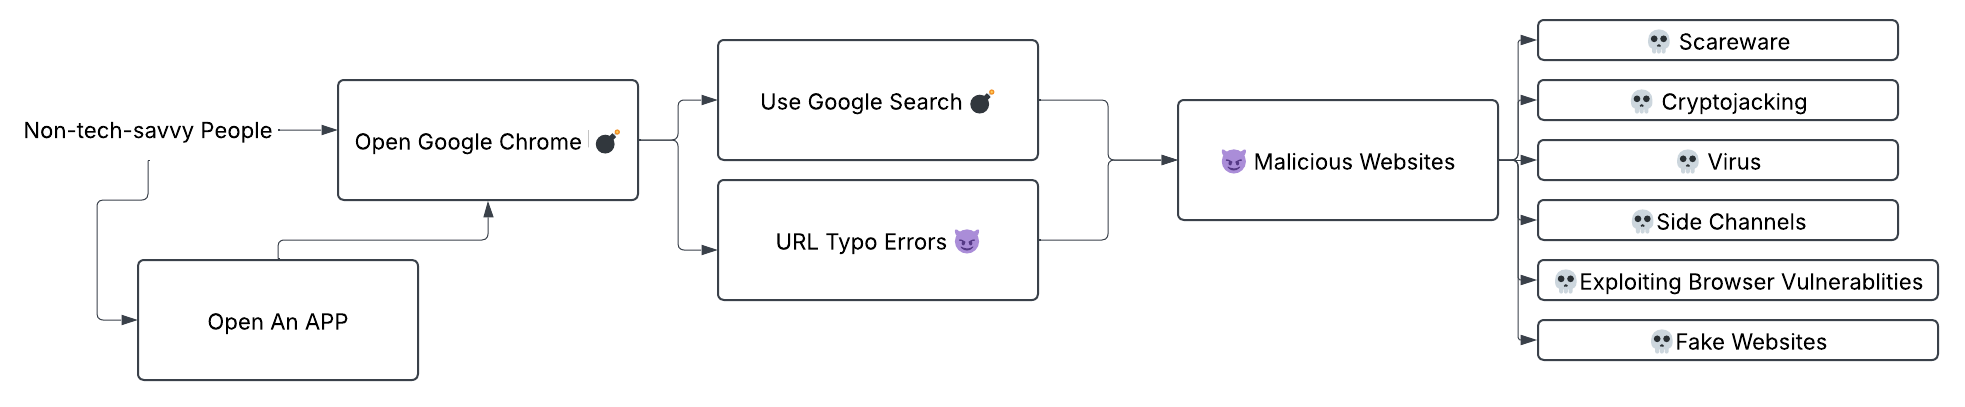
\includegraphics[width=1\textwidth]{threatmodel.png}
\caption{Threat Model: Browsers and Search Engines Considered Unsafe}
\label{fig:threat_model} % Label for referencing the image in the paper
\end{figure*}
%%%%%%%%%%%%%%%%%%%%%%%%%%%%%%%%%%%%%%%%%%%%%%%%%%%%%%%%%%%%%%%%%%%%%%%%%%%%%%%%
\section{Design}
\label{sec:methodology}

The purpose of the S/P mode is to create a distinct separation between simple users and power users. This section details the design of the S/P mode toggle. Each Windows user account would offer the S/P mode toggle directly on the login screen. This toggle does not alter the existing permission management systems of Windows or Unix-based operating systems.

\autoref{fig:demo_image} presents a prototype of the proposed login screen UI incorporating the S/P mode toggle. The key modification compared to the standard Windows login screen is the addition of a new button located on the right side of the existing login options. This button allows users to directly select either S Mode or P Mode from the login interface. The system remembers the user’s previous choice: if S Mode was selected during the last session, it will default to S Mode; likewise, if P Mode was chosen, it will default to P Mode unless the user opts to switch. Notably, this enhancement is strictly a UI-level adjustment and does not alter the underlying functionality for user accounts, whether they are administrators, sudo users, or regular users. Instead, it introduces a secure and intuitive interface to complement the existing account structure without changing the way users interact with the system. When the user selects S Mode, the operating system does not launch the standard desktop UI. Instead, it uses Microsoft Edge as the engine for running PWAs and presents a UI similar to iPhone or Android, where users can access and launch PWAs in an intuitive, app-like interface. This design enhances accessibility while maintaining the simplicity of the PWA-focused environment.

\begin{figure}[t] % Use figure* for full-width images in two-column layouts
\centering
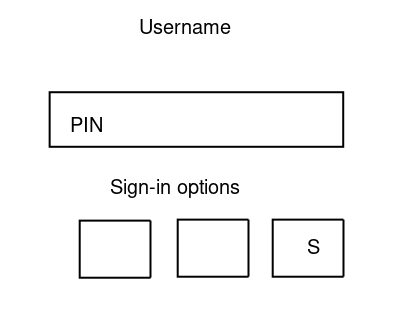
\includegraphics[width=0.4\textwidth]{demo.jpg} % Set to full text width
\caption{Demo of the S/P Mode Toggle Login Screen}
\label{fig:demo_image}
\end{figure}


\subsection{S Mode}

\autoref{fig:smodearch} illustrates the architecture diagram for the S Mode toggle, while \autoref{fig:walledgarden} depicts the scope of the PWA Walled Garden. S Mode is specifically designed for users who focus on essential tasks such as working with Word, Excel, or engaging with social media apps like YouTube and Instagram, supported through progressive web apps. Advanced functionalities intended for power users are omitted in this environment. The primary goal of S Mode is to implement stringent controls, with restrictions surpassing those enforced on iPhones in numerous settings.

\begin{figure}[h!]
\centering
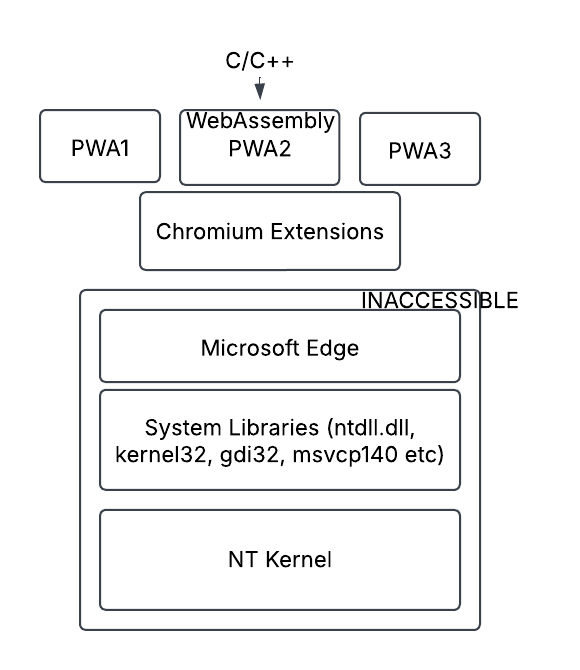
\includegraphics[width=0.4\textwidth]{smodearch.png}
\caption{S Mode Toggle Architecture (NOT Windows S mode)}
\label{fig:smodearch} % Label for referencing the image in the paper
\end{figure}

\begin{figure*}[h!]
    \centering
    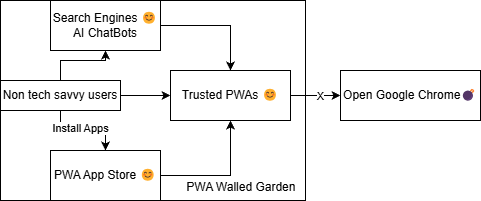
\includegraphics[width=0.6\linewidth]{walledgarden.png}
    \caption{PWA Walled Garden in S Mode Toggle (NOT Windows S mode)}
    \label{fig:walledgarden}
\end{figure*}

\subsubsection{Disallow Direct Browser Use}

Browsers are considered unsafe and are strictly prohibited for direct use. They are only permitted for hosting PWAs. No application, including Microsoft Edge or third-party browsers like Google Chrome and Firefox, should provide standalone browser functionalities.

\subsubsection{Disallow Direct Search Engine Use}

Search engines are also regarded as unsafe and are disallowed in S Mode. This restriction helps prevent phishing attempts, blocks access to fake websites, and mitigates the growing issue of SEO pollution\cite{10.1007/978-3-031-56063-7_4}. Users are limited to searching only within the websites of installed PWAs, and are encouraged to rely on AI-powered chatbots, such as Microsoft Copilot, ChatGPT, or Deepseek, for accessing web content securely.

\subsubsection{Browser Running Within the App Sandbox in S Mode}

In S Mode, the browser application itself should operate within the App Sandbox\cite{MicrosoftAppIsolationOverview} to add an additional layer of defense. This setup ensures that PWAs are not only sandboxed by the browser but also benefit from the security of the App Sandbox encapsulating the browser. This dual-layer protection strengthens security by combining the isolated environments of both the browser and the App Sandbox.

\subsubsection{All Progressive Web Apps Must Be Installed via the App Store}

Progressive web apps are installed in a manner similar to traditional apps on platforms like Google Play Store or Apple App Store. However, instead of native apps, users install PWAs. These apps run internally using Microsoft Edge, but direct access to the browser itself is restricted.

\subsubsection{Browser Extensions are in the App Store}

Since PWAs operate within browsers, they often leverage browser extensions. For example, users might install ad blockers for YouTube PWAs or use global speed/pitch adjusters to modify playback speeds for apps like Spotify, transforming them into nightcore players. To maintain control, such extensions should be made available only through the App Store.

\subsubsection{Restrict Direct URL Access}

Allowing users to type URLs poses risks, as typographical errors can lead to security issues. Hence, direct URL access is prohibited in all forms within S Mode.

\subsubsection{PWA App Store Must Be Open}

Progressive Web Apps are web resources and should remain open to ensure accessibility and transparency. Developers should have the ability to submit their PWAs to a publicly available GitHub repository, akin to how Microsoft vcpkg operates, or alternatively, rely on web standards to oversee PWA App Stores. Furthermore, no commission fees should be allowed for app submissions. This openness enables other operating systems, such as Linux and macOS, to adopt and implement this security model effectively.

\subsubsection{Limit External Links}

Web pages often include external links that could redirect users to malicious websites. To address this, PWAs must include a manifest file specifying a whitelist of allowed external links. By default, login pages for services like Google, Apple, or Microsoft accounts are permitted unless explicitly restricted by the app.

\subsubsection{Restrict Permission Changes}

Modern apps frequently request excessive permissions to exploit user data. In S Mode, users are prohibited from modifying app permissions to maintain data security.

\subsubsection{Disallow Sideloading}

Sideloading of both PWAs and browser extensions is strictly prohibited in S Mode.

\subsubsection{Restrict Basic Settings Changes}

Even seemingly simple settings, like date and time or timezone configurations, can be problematic for users. Incorrect settings often disrupt app functionality, such as the Google Play Store. To reduce complexity and maintenance needs, these settings cannot be altered in S Mode.

\subsubsection{Restrict File Access to \texttt{\$HOME/.smode} Directory}

Complete restriction of file access is impractical, yet unrestricted access poses significant risks, as demonstrated by historical issues with Windows Phone. In S Mode, file access is limited to the \texttt{\$HOME/.smode} directory (\%USERPROFILE\%/.smode on Windows), ensuring essential functionality while minimizing potential vulnerabilities. Additionally, users can synchronize their data seamlessly with Microsoft OneDrive within S Mode. However, apps should NEVER be allowed to access Microsoft OneDrive directly to prevent ransomware.

\subsubsection{App Transitions Restricted to Installed PWAs}

If one PWA attempts to open another PWA, the transition must be limited to installed PWAs. A browser popup should appear to handle the transition, but if the target PWA is not installed, the app transition should be blocked.

\subsubsection{Gradually Implement Enhanced Security Measures for PWAs}

Progressive Web Apps should gradually adopt stronger security measures to improve their robustness. For instance, WebAssembly binaries—often compiled from memory-unsafe languages like C/C++—require additional mitigations, such as WebAssembly Memory Tagging\cite{webassemblymemorytagging}, to ensure safer execution. S Mode offers an opportunity to enforce stricter security measures for PWAs. However, as most WebAssembly applications currently lack adequate mitigations, this process must be introduced incrementally to allow for widespread adoption and compatibility.

\subsubsection{S Mode UI Should Closely Resemble iPhone's UI}

The iPhone's UI has become the de facto standard for mobile phone interfaces and walled garden operating systems. As mobile UIs are the most familiar to a majority of end users, adopting a similar design for S Mode ensures ease of use and eliminates any learning curve for users. 

\subsubsection{Automatic PWA Synchronization}

Currently, PWAs are synchronized through Microsoft Edge, making them easily accessible for end users. To enhance usability in S Mode, these PWAs should be automatically synced, ensuring a seamless experience for users.

\subsubsection{Integration with Trusted Platform Module for Sensitive Apps}

Sensitive PWAs, such as the Chase Bank App, can enhance security by leveraging the Trusted Platform Module\cite{10.1145/3320269.3372197} to verify the integrity of both the Edge browser engine and the banking application's code. This ensures that sensitive operations are executed within the app's sandbox, with their integrity fully guaranteed.

\subsection{P Mode}

P Mode represents the Windows environment in its standard form. It allows users to perform tasks such as running \texttt{.exe} files, utilizing browsers, accessing the Windows Subsystem for Linux, using \texttt{cmd} and PowerShell, editing the registry (\texttt{regedit}), and rebooting into UEFI to install other operating systems. Logging into P Mode signifies that the user is a power user, comparable to utilizing \texttt{unsafe} blocks in programming languages like C\# or Rust. It conveys to the operating system: "I understand the risks and am fully capable of managing them. Please grant me unrestricted access to perform my tasks."

With the introduction of the S/P mode toggle, P Mode also takes on the responsibility of managing settings for S Mode. Below, we present the design principles for P Mode.

The Windows Settings app in P Mode should include a dedicated section for managing S Mode settings.

\subsubsection{Power User Mode Must Grant Full Control, Including Installation of Other Operating Systems}

P Mode is designed for power users and is not intended to be a locked-down environment. Power users should not face the restrictions common to ecosystems like Android or iOS. Instead, P Mode must allow users complete freedom, including the ability to install alternative operating systems.

\subsubsection{Enable Comprehensive Settings Management}

While S Mode restricts changes to date, time, and timezone settings, P Mode must provide full access to these configurations. This highlights the versatility of the S/P mode toggle compared to fully locked platforms like iPhones, where errors in settings can arise due to the absence of boundaries for unsafe operations. In the pursuit of complete safety, unintended vulnerabilities may emerge—this toggle offers a balance.

\subsubsection{Allow Sideloading of PWAs and Browser Extensions into S Mode}

Since PWAs are essentially websites, sideloading them into S Mode should be straightforward—users can simply input URLs to initiate the process. Additionally, the Edge browser in P Mode can feature an option that allows users to install PWAs and Chromium extensions directly into S Mode.

\subsubsection{Centralized Permission Management for PWAs in S Mode}

Permissions for PWAs in S Mode should be managed exclusively through P Mode. Android apps often manipulate users into granting unnecessary permissions. By centralizing permission management in P Mode, this approach protects non-tech-savvy users from being tricked by applications while retaining full functionality for power users.

\subsubsection{Adjust PWA Synchronization Settings}

P Mode should offer users the flexibility to customize how PWAs are synchronized for S Mode. This ensures personalized and efficient use of PWAs.

\subsubsection{Modify File Access Settings for S Mode}

By default, file access in S Mode is restricted to \texttt{\$HOME/.smode} (On Windows it is \texttt{\%USERPROFILE\%/.smode}) directory. In P Mode, users should be able to expand access by adding more directories or modifying the default directory that S Mode can access.

\subsubsection{Dedicated File Storage for Each PWA}

In addition to shared storage for Progressive Web Apps, each PWA can maintain its own dedicated file storage. This approach enhances sandboxing capabilities in S Mode, ensuring greater isolation and security for individual app.

\subsubsection{Popup Suggestions for Entering S Mode in Sensitive Apps}

Sensitive applications, such as banking PWAs like Chase, require heightened security measures. In this context, browsers operating in power user mode should provide a discreet suggestion prompting users to switch to S Mode for enhanced protection. To ensure a seamless user experience, these prompts should be limited in frequency and appear only for sensitive applications. Unless mandated by a bank's policy to enforce the use of S Mode, these suggestions should remain optional, allowing users to make the choice without feeling overwhelmed by intrusive notifications.

\subsubsection{Gradually Expand Options for Modifying S Mode Settings}

The aforementioned list outlines initial options for modifying S Mode settings. Over time, users may require additional flexibility, such as changing the browser engine used for PWAs instead of relying solely on Microsoft Edge. However, this introduces potential security risks—if the browser engine originates from a malicious source, it could compromise the entire system, as illustrated by scenarios like using a Chase Bank PWA. To mitigate these risks, modifications should only be allowed through the App Store in P Mode or by requiring cryptographic signatures provided by Microsoft to verify the integrity of the browser engine. These changes must be implemented with caution and gradually.

Additional options, such as enabling the sideloading of Win32 sandbox applications into S Mode, could pose significant security risks. Unfortunately, many apps vendors—such as WeChat—choose to monetize user data rather than offering PWAs. To ensure the security and integrity of S Mode, these features must be implemented thoughtfully and incrementally. Nonetheless, Progressive Web Apps should remain the preferred method for app delivery over Win32 sandbox applications, as PWAs inherently add an extra layer of sandboxing through the browser engine.

%%%%%%%%%%%%%%%%%%%%%%%%%%%%%%%%%%%%%%%%%%%%%%%%%%%%%%%%%%%%%%%%%%%%%%%%%%%%%%%%
\section{Evaluation}
\label{sec:eval}

This is a position paper, so direct evaluation through the implementation of this feature and subsequent data collection on its impact on the Windows security ecosystem is not feasible.

However, extensive evaluations can still be conducted indirectly. For example, comparisons can be made regarding security, performance, and usability relative to existing operating system modes. Other related studies provide valuable data that support and demonstrate the effectiveness.


\subsection{App Size}

Progressive Web Apps offer a significant advantage in terms of their smaller binary size compared to Android and iOS applications, a fact supported by various studies and statistics. This advantage stems from two primary factors. First, the browser itself provides numerous built-in functionalities, eliminating the need for individual apps to duplicate code to implement those features. Second, and more importantly, PWAs are essentially websites or web pages. As a result, browsers only download the specific use-case a user requires, unlike Android or iOS apps, which often include features that the user never uses\cite{TheWebIsDead}.

\textit{The Web Is Dead! Long Live The Web! }\cite{TheWebIsDead} by Sam Thorogood highlighted a notable comparison in 2018: the Twitter app on iOS required 186MB, on Android 70MB, while the Twitter Progressive Web App was under 2MB, demonstrating the significant size advantage of PWAs.

The benefits of Progressive Web Apps extend beyond Twitter. According to Microsoft's documentation\cite{MicrosoftEdgePWAs}, Tinder experienced remarkable improvements with its PWA, reducing load times from 11.91 seconds to 4.68 seconds. Additionally, the PWA's size is 90\% smaller compared to the compiled Android app, showcasing its efficiency.

PWAs are consistently smaller in size compared to Android and iOS apps. While certain applications, such as games, may have smaller native versions, developers still have the option to create Win32 sandbox apps for S Mode. Additionally, P Mode remains available, allowing users to access traditional Win32 applications as needed.

\subsection{Security Evaluation}

\autoref{tab:security_comparison} highlights the security measures of the S/P Mode Toggle compared to other operating systems. The S/P Mode Toggle demonstrates notable security advantages over Android and iOS. Under S Mode, the system is significantly more restricted, with features such as the prohibition of direct browser use and the unavailability of numerous settings, ensuring a more locked-down environment. While P Mode is less secure, S Mode offers a reliable solution for non-tech-savvy users or professionals in corporate settings who primarily perform lightweight tasks such as working with Word, Excel, or PowerPoint. For these users, adhering to S Mode provides a strong assurance of a trouble-free experience without the need to transition to P Mode.

S mode toggle uses Progressive Web Apps which are inherently sandboxed by the browser—a system designed as a natural sandbox. This structure offers a higher level of security compared to iOS apps. Furthermore, the browser operates as a WebAssembly virtual machine, allowing memory-unsafe C/C++ applications to run securely within the browser environment. Advanced security mitigations, such as \textit{WebAssembly Memory Tagging}\cite{webassemblymemorytagging}, enhance protection against vulnerabilities. Implementing such mitigations is significantly more challenging with native applications on Android and iOS.

Another significant advantage is the ease of upgrading every component of the system. This includes the app itself, the browser, and the operating system. When any of these components are patched, the system becomes inherently safer. Additionally, since Progressive Web Apps are fundamentally websites, addressing vulnerabilities or implementing feature updates is significantly faster compared to native apps. Moreover, updates for PWAs do not require app store approval, streamlining the process even further.

The S Mode toggle also minimizes the risk of SEO pollution by restricting search engines to only retrieve information from trusted apps. This feature offers a distinct advantage over Android and iOS, as their apps are not inherently SEO-friendly, making such a controlled search experience unattainable. As a result, Android and iOS systems expose non-tech-savvy users to a higher risk of encountering fraudulent content, whereas S Mode provides enhanced protection.


\begin{table*}[h!]
\caption{Comparison of Security Across S/P Mode, Android, iOS, and Windows.}
\centering
\begin{tabular}{@{}p{4cm}p{3cm}p{3.5cm}p{2.5cm}p{3cm}@{}}
\toprule
\textbf{Security}                  & \textbf{S/P Mode}                            & \textbf{Android}             & \textbf{iOS}                  & \textbf{Windows}             \\
\midrule
User Mode Separation              & \cmark\ (S Mode for basic users, P Mode for power users) & \xmark\ (No separation)      & \xmark\ (No separation)       & \cmark\ (Admin/User accounts) \\
App Restrictions                  & \cmark\ (Only via official store, no sideloading)  & \xmark\ (Sideloading supported) & \cmark\ (Only via App Store)   & \xmark\ (Manual installation allowed) \\
Browser Restrictions              & \cmark\ (Browser and search disabled, PWA-only access) & \xmark\ (Full browser access)   & \xmark\ (Full browser access)  & \xmark\ (Full browser access) \\
File Access Restrictions          & \cmark\ (Restricted to \texttt{\$HOME/.smode} directory) & \xmark\ (Varies by device)      & \cmark\ (Strict sandboxing)    & \xmark\ (Full file access)    \\
Permission Management             & \cmark\ (Centralized in P Mode)                   & \xmark\ (Managed per app)       & \cmark\ (Strict prompts)       & \xmark\ (Scattered permissions) \\
Update Flexibility                & \cmark\ (Independent OS and browser updates)      & \xmark\ (Highly fragmented)     & \cmark\ (Unified updates)      & \cmark\ (Separate OS/browser updates) \\
Operating System Updates          & \cmark\ (Frequent updates with patches and features) & \xmark\ (Delayed, depends on vendors) & \cmark\ (Regular and unified) & \cmark\ (User-controlled update strategies) \\
Sideloading Restrictions                 & \cmark\ (Prohibited in S Mode, allowed in P Mode)  & \xmark\ (Widely supports sideloading) & \cmark\ (Strictly prohibited)  & \xmark\ (Fully supports sideloading) \\
Search Engine Restrictions        & \cmark\ (Search limited to installed PWA content)  & \xmark\ (Unlimited search)      & \xmark\ (Unlimited search)     & \xmark\ (Unlimited search)    \\
Browser Security Updates          & \cmark\ (Frequent updates for enhanced protection) & \cmark\ (Depends on the user)   & \cmark\ (Unified control)      & \cmark\ (User-controlled updates) \\
Setting Restrictions              & \cmark\ (Time and timezone changes disabled)      & \xmark\ (Fully adjustable)      & \cmark\ (Partial restrictions) & \xmark\ (No unified restrictions) \\
App Sandbox Restrictions          & \cmark\ (Each app runs in its own sandbox)        & \xmark\ (Inconsistent sandboxing) & \cmark\ (Strict sandboxing)    & \xmark\ (Some apps lack sandbox) \\
Prohibit Executable Files         & \cmark\ (Blocked in S Mode, allowed in P Mode)    & \cmark\ (Executables not supported) & \cmark\ (Strictly prohibited)  & \xmark\ (Executable files allowed) \\
Ban on Untrusted External Links   & \cmark\ (Only allows links to installed PWAs; user confirmation required) & \xmark\ (Unrestricted external links) & \xmark\ (Unrestricted external links) & \xmark\ (Unrestricted external links) \\
Side-Channel Mitigations          & \cmark\ (PWAs only from trusted sources; no side-channel risks) & \xmark\ (Susceptible to side-channel risks) & \xmark\ (Partial mitigations) & \xmark\ (Varies by app/system) \\
Cryptojacking Protection & \cmark\ (No mining due to PWA restrictions)    & \xmark\ (Potentially vulnerable)  & \xmark\ (Open via web browsers) & \xmark\ (Depends on installed apps) \\
Scareware Protection              & \cmark\ (PWAs vetted through trusted sources)    & \xmark\ (Vulnerable due to open ecosystem) & \xmark\ (Open via web browsers) & \xmark\ (Users must verify software) \\
Memory Safety Mitigations         & \cmark\ (Incremental measures like WebAssembly Memory Tagging) & \xmark\ (Highly dependent on OS/app implementation) & \xmark\ (Potential kernel exploits from buggy apps) & \xmark\ (Memory safety depends on developer practices) \\
\bottomrule
\end{tabular}
\label{tab:security_comparison}
\end{table*}

\subsection{Usability Evaluation}

\autoref{tab:usabilitycomparison} provides a usability comparison table. When evaluated alongside Android and iOS, the S/P Mode toggle showcases significant usability advantages. As a simple UI feature integrated into the login screen, the S/P Mode toggle does not alter the way the operating system functions. Users retain the ability to replace their operating systems seamlessly, as they currently can, which is not easily achievable on Android or iOS. Moreover, in P Mode, users can run Win32 .exe PE executables—a feature that is unavailable on iOS. While Android permits some degree of this functionality through Termux, the operating system itself imposes limitations, and running graphical binaries is considerably more challenging compared to Windows.

Additionally, the S/P Mode toggle enhances usability for non-tech-savvy users by providing a secure and simplified experience in S Mode. This eliminates concerns about malware or complex system details, giving these users the opportunity to focus on learning to use a computer safely before transitioning to P Mode.

Chromium extensions significantly enhance usability compared to Android and iOS apps in our S mode toggle. Chromium-based extensions enable extensive customization options for apps, far surpassing the capabilities of Android and iOS. Additionally, browser functionalities on Android are more limited than those on Windows; for instance, Google Chrome on Android lacks support for extensions. While Microsoft Edge now offers extension support on Android, this feature remains unavailable on iOS, further highlighting the advantages of browser-based customization in S Mode.

The developer experience in our S/P Mode far surpasses that of proprietary software development on platforms like Android and iOS. The web operates as an open standard, enabling developers to compile C/C++ code into WebAssembly and run it seamlessly across all platforms. In contrast, Android and iOS impose restrictions on the programming languages developers can easily use and require separate development efforts for each platform. With S/P Mode, developers benefit from using PWAs in S Mode or Win32 APIs in P Mode—both of which are well-established, widely understood, and fully supported by mainstream platforms (Win32 APIs are compatible through wine).

From a usability perspective, comparing our S/P Mode toggle to Windows S Mode reveals significant limitations in the latter. Windows S Mode lacks apps, and once users switch out of it, there is no option to revert back. Furthermore, it fails to protect users from scams originating from Microsoft Edge and Bing. Additionally, it offers no safeguards for power users, as they cannot utilize Windows S Mode effectively. It also does not prevent users from accidentally altering critical settings like date and time. In contrast, our S/P Mode toggle stands out with its high level of customization, making it versatile and suitable for both simple users and power users, addressing a broad range of use cases with tailored solutions.

\begin{table*}[h!]
\caption{Usability Comparison: S/P Mode, Android, iOS, Windows S Mode, and Standard Windows}
\centering
\begin{tabular}{@{}p{2cm}p{2cm}p{3cm}p{3cm}p{3cm}p{3cm}@{}}
\toprule
\textbf{Usability}                    & \textbf{S/P Mode}                        & \textbf{Android}                  & \textbf{iOS}                     & \textbf{Windows S Mode}           & \textbf{Windows}                  \\
\midrule
Operating System Replacement Support & \cmark\ (Full control, OS replacement possible) & \xmark\ (Hardware restrictions, nearly impossible)  & \xmark\ (Completely closed, no OS replacement)   & \xmark\ (Requires exiting S Mode) & \cmark\ (Open but limited by hardware compatibility) \\
Mode Switching                        & \cmark\ (Seamless switching between S and P Mode) & \xmark\ (No mode switching)       & \xmark\ (No mode switching)       & \xmark\ (Cannot switch without exiting S Mode) & \cmark\ (Supports admin and user switching)          \\
Application Installation Options      & \cmark\ (Supports official store, PWA, and sideload in P Mode) & \cmark\ (Supports store, APK, and sideloading) & \xmark\ (Restricted to App Store apps) & \xmark\ (Restricted to Microsoft Store apps) & \cmark\ (Supports store and sideloading)             \\
File Access                           & \cmark\ (S Mode restricts directories, P Mode allows full access) & \cmark\ (Supports sandbox and external access)   & \xmark\ (Strict sandbox restrictions)  & \xmark\ (Limited access to system directories) & \cmark\ (Full file access)                           \\
Web Browsing Support                  & \cmark\ (S Mode disables browser, P Mode supports full browser) & \cmark\ (Powerful, open browser support) & \cmark\ (Browser supported with limitations) & \xmark\ (Restricted to Microsoft Edge) & \cmark\ (Full browser functionality supported)       \\
Settings Flexibility                  & \cmark\ (S Mode restricts critical settings, P Mode allows customization) & \cmark\ (Full user control)       & \xmark\ (Partially restricted)     & \xmark\ (Strict restrictions on changing settings) & \cmark\ (Complete customization freedom)            \\
Application Exclusivity               & \cmark\ (PWA in S Mode, compatible across platforms) & \xmark\ (Applications limited to Android devices) & \xmark\ (Applications limited to iOS devices) & \xmark\ (Applications limited to Windows environment) & \cmark\ (Supports applications across environments)  \\
Application Update Method             & \cmark\ (Developers update directly, no app store required) & \xmark\ (Dependent on app store updates) & \xmark\ (Must go through App Store) & \xmark\ (Requires Microsoft Store for updates) & \cmark\ (Supports direct updates by developers)      \\
Programming Language Support          & \cmark\ (Supports WebAssembly, compatible with C++) & \xmark\ (Primarily Java/Kotlin)  & \xmark\ (Primarily Objective-C/Swift) & \xmark\ (Limited frameworks and language support) & \cmark\ (Supports diverse languages including C++)   \\
\bottomrule
\end{tabular}
\label{tab:usabilitycomparison}
\end{table*}

\subsection{Performance evaluation}

\autoref{tab:performance_comparison} presents the performance evaluation of the S/P Mode. Compared to traditional Windows setups, one notable advantage is that PWAs, being web pages, benefit from Microsoft Edge's smart sleep functionality, which is the most power efficient compared to other browsers on Windows\cite{DigitalCitizenBatteryTest}. Microsoft Edge puts background web pages into sleep mode\cite{MicrosoftEdgeSleepingTabs, MicrosoftEdgePerformance}—a feature not feasible for Win32 applications, as standard C/C++ binaries lack built-in support for app suspension. Consequently, the OS kernel must save the entire state when the user closes the lid. When users logins with the S Mode instead of P Mode, the system becomes significantly lightweight as it exclusively runs Progressive Web Apps. This design enhances Windows' power efficiency for lightweight tasks, surpassing the power efficiency of traditional Win32 configurations.

In contrast to Android and iOS, PWAs in S Mode utilize the shared Edge browser engine, while P Mode takes advantage of shared Windows DLLs across various applications, as it functions like standard Windows. This architectural design ensures performance benefits optimized for each mode. Additionally, S/P Mode offers superior resource sharing in both S and P modes, unlike Android and iOS apps, where each app operates within a separate app sandbox.

\begin{table*}[h!]
\caption{Performance Comparison: S/P Mode, Android, iOS, Windows S Mode, and Standard Windows}
\centering
\begin{tabular}{@{}p{2cm}p{2cm}p{3cm}p{3cm}p{3cm}p{3cm}@{}}
\toprule
\textbf{Performance}       & \textbf{S/P Mode}                        & \textbf{Android}                  & \textbf{iOS}                     & \textbf{Windows S Mode}           & \textbf{Windows}                  \\
\midrule
Resource Usage                      & \cmark\ (PWA is lightweight, downloads only necessary content) & \xmark\ (Applications depend on virtual machine, leading to inefficiency) & \xmark\ (Applications tend to be larger due to high-resolution assets) & \xmark\ (Applications have higher local storage requirements) & \cmark\ (Shared system resources reduce redundancy) \\
Performance Optimization            & \cmark\ (WebAssembly provides near-native performance)          & \xmark\ (Java virtual machine introduces performance bottlenecks)       & \cmark\ (Native code delivers stable performance)                      & \xmark\ (Optimizations depend on app development quality)    & \cmark\ (Optimization depends on developer and hardware)     \\
Background Sleep Support            & \cmark\ (PWA pages naturally sleep when inactive)               & \xmark\ (Some apps have frequent background activity)                  & \xmark\ (Apps must be tailored for sleep modes)                       & \xmark\ (Most apps cause significant background energy drain) & \xmark\ (Apps must be specifically modified to fully sleep)  \\
Energy Consumption                  & \cmark\ (Unified browser manages resources efficiently, reducing power draw) & \xmark\ (Energy usage depends on app and device quality)              & \xmark\ (Sandbox environment adds resource overhead)                  & \xmark\ (Background resources are not fully optimized)        & \xmark\ (Energy draw varies without unified management)       \\
Shared Resource Model               & \cmark\ (Browser provides shared pool for all PWA applications) & \xmark\ (Sandbox applications rarely share resources)                 & \xmark\ (Sandbox isolates application resources)                     & \xmark\ (Applications are isolated, with no shared mechanism) & \cmark\ (Applications share system resources effectively)     \\
Update Impact                       & \cmark\ (Only relevant content is updated, reducing resource strain) & \xmark\ (Full updates require downloading large packages)             & \xmark\ (System updates tend to bundle unnecessary data)             & \xmark\ (System updates cause significant overhead)           & \xmark\ (Update impact depends on user management)            \\
\bottomrule
\end{tabular}
\label{tab:performance_comparison}
\end{table*}

\subsection{Deployment Evaluation}

\autoref{tab:sp_vs_group_policies} presents a comparison between the S/P Mode toggle and Windows Group policies. Unlike traditional tools such as Windows administrative group policies, the S/P Mode toggle is designed with simplicity in mind, making it highly accessible to average users. By merely switching to S Mode, users can enable a secure, locked-down walled garden environment without requiring additional configurations. While group policies can achieve comparable results, their complexity necessitates an IT administrator, posing challenges for non-tech-savvy individuals who purchase computers from retail stores like Walmart or Best Buy. The S/P Mode toggle eliminates this barrier, offering an intuitive solution that ensures system security with minimal effort.

This model offers additional deployment advantages, as it is compatible with all existing operating systems, including Linux and macOS. Users of Linux, macOS, or even future operating systems can seamlessly benefit from the S/P Mode toggle, enjoying both enhanced security and improved usability without sacrificing any current functionalities. Progressive Web Apps seamlessly operate on Linux today without any complications. This is because the web serves as a universal platform that is inherently platform-agnostic, ensuring compatibility across various operating systems. Moreover, the simplicity of this model allows individual users to deploy it independently, eliminating the need to rely on an IT professional for setup.

\begin{table*}[h!]
\centering
\caption{Comparison: S/P Mode Toggle vs. Windows Group Policies}
\begin{tabular}{@{}p{4.5cm}p{5.5cm}p{5.5cm}@{}}
\toprule
\textbf{Feature}                      & \textbf{S/P Mode Toggle}                     & \textbf{Windows Group Policies}              \\
\midrule
Configuration Method                  & Simple toggle between S Mode and P Mode via user interface, designed for all users & Configured through administrative tools like gpedit.msc or Active Directory, requiring technical expertise \\
Target Audience                       & Everyday users (S Mode) and advanced users (P Mode)                                & IT professionals and system administrators managing organizational environments \\
Implementation Complexity             & \cmark\ (User-friendly, minimal setup required; no technical knowledge needed)     & \xmark\ (Highly complex, configuration requires expertise, not suitable for non-tech-savvy users) \\
Dynamic Adjustment                    & \cmark\ (Users can instantly switch between S and P Mode based on needs)           & \xmark\ (Requires admin approval and pre-configuration; adjustments are not user-initiated) \\
Scope of Control                      & Individual user-level settings (toggle per device)                                 & Organization-wide enforcement across multiple devices and users \\
Feature Granularity                   & Limited to mode-based controls (e.g., app installation, resource access)           & Highly granular (controls registry, software restrictions, network policies, etc.) \\
Ease of Rollback                      & \cmark\ (Instantly revert back to S Mode)                                          & \xmark\ (Rollback requires manual reconfiguration or scripts, not easy for average users) \\
Security Management                   & \cmark\ (Switch to P Mode for flexibility; back to S Mode for strict controls)      & \cmark\ (Powerful organizational security enforcement, but complex to implement) \\
Admin Rights Requirement              & \xmark\ (No admin privileges needed for toggling modes)                            & \cmark\ (Admin rights are mandatory for setup, changes, and enforcement) \\
Usability for Everyday Users          & \cmark\ (Ideal for non-technical users who rely on basic apps like Word/Excel)      & \xmark\ (Overwhelming and inaccessible for users who only need basic functionality) \\
Usage Scalability                     & Best suited for single-user or device-level control                                 & Designed for enterprise-level deployments, not casual individual usage \\
Integration with External Systems     & \cmark\ (Integrates with cloud services, PWAs support APIs for external communication) & \cmark\ (Extensive integration with Windows Server, Azure AD, enterprise tools) \\
\bottomrule
\end{tabular}
\label{tab:sp_vs_group_policies}
\end{table*}
\section{Related Work}

\textit{Dynamic Malware Analysis in the Modern Era--A State of the Art Survey}\cite{10.1145/3329786}, authored by Or-Meir, Ori, Nissim, Nir, Elovici, Yuval, and Rokach, Lior, provides a definition of malware and categorizes it into various types, including viruses, trojans, spyware, worms, adware, scareware, bots, ransomware, and cryptominers. The paper also classifies malicious behaviors associated with malware. It offers a comprehensive survey evaluating the strengths and weaknesses of different analysis methods and their resilience against malware evasion techniques. In addition, the authors highlight how mainstream approaches predominantly rely on machine learning for malware detection.
The paper \textit{Analysis of Machine learning Techniques Used in Behavior-Based Malware Detection} by Firdausi, Ivan, Lim, Charles, Erwin, Alva, and Nugroho, Anto Satriyo employed the J48 decision tree algorithm, achieving a recall of 95.9\%, a false positive rate of 2.4\%, a precision of 97.3\%, and an accuracy of 96.8\%. \textit{Malware Classification with Recurrent Networks}\cite{7178304} by Pascanu, Razvan, Stokes, Jack W., Sanossian, Hermineh, Marinescu, Mady and Thomas, Anil explored malware detection using a recurrent bidirectional neural network to analyze system calls, with their best model yielding a precision of 82\% and a false positive rate of 0.5\% based on 114 distinct system calls from 250,000 malware samples. \textit{A Machine-Learning Approach for Classifying and Categorizing Android Sources and Sinks}\cite{rasthofer2014machine} by Rasthofer, Siegfried, Arzt, Steven, and Bodden, Eric proposed the SUSI framework, evaluated on 11,000 malware samples, with their top-performing model achieving an accuracy of 92.3\%. \textit{Adaptive Detection of Covert Communication in HTTP Requests}\cite{6377758} by Schwenk, Guido and Rieck, Konrad analyzed 695 malware samples but did not report metrics such as accuracy, precision, or false positive rate. \textit{Trusted System-Calls Analysis Methodology Aimed at Detection of Compromised Virtual Machines Using Sequential Mining}\cite{10.1016/j.knosys.2018.04.033} by Nissim, Nir, Lapidot, Yuval, Cohen, Aviad and Elovici, Yuval utilized memory dumps from virtual machines and reconstructed systems using WinDbg; their analysis of ten malware and six benign samples with random forest achieved a precision rate of 98\% with no false positives. \textit{Machine Learning in Side-Channel Analysis: A First Study}\cite{hospodar2011machine} by Hospodar, Gabriel, Gierlichs, Benedikt, De Mulder, Elke, Verbauwhede, Ingrid and Vandewalle, Joos demonstrated that machine learning could effectively extract cryptographic keys using power consumption traces as features, with their LS-SVM linear classifier reaching a success rate of 75\%. \textit{On the Feasibility of Online Malware Detection with Performance Counters}\cite{10.1145/2508148.2485970} by Demme, John, Maycock, Matthew, Schmitz, Jared, Tang, Adrian, Waksman, Adam, Sethumadhavan, Simha, and Stolfo, Salvatore tested their decision tree-based implementation on Android and Linux, using 201 benign samples and 503 malware samples, achieving a detection rate of 83\% and a false positive rate of 10\%. Finally, \textit{EDDIE: EM-Based Detection of Deviations in Program Execution}\cite{10.1145/3079856.3080223} by Nazari, Alireza, Sehatbakhsh, Nader, Alam, Monjur, Zajic, Alenka and Prvulovic, Milos monitored electromagnetic emissions from embedded and IoT devices, detecting statistical anomalies caused by code injections into application loops.

\textit{Understanding and Detecting Real-World Safety Issues in Rust}\cite{10.1145/3385412.3386036} by Qin, Boqin, Chen, Yilun, Liu, Haopeng, Zhang, Hua, Wen, Qiaoyan, Song, Linhai, and Zhang, Yiying highlights that programming languages like Rust can encounter memory safety issues if the \texttt{unsafe} keyword is misused. The authors conducted an extensive study, analyzing five widely-used Rust libraries and two online security databases. Their manual inspection uncovered 70 memory bugs, 100 concurrency bugs, and 110 programming errors leading to panics. This research emphasizes that excessive reliance on \texttt{unsafe} significantly diminishes its intended effectiveness.

\textit{Is Google Getting Worse? A Longitudinal Investigation of SEO Spam in Search Engines}\cite{10.1007/978-3-031-56063-7_4} by Bevendorff, Janek, Wiegmann, Matti, Potthast, Martin, and Stein, Benno examines the decline in Google Search quality due to the rise of SEO spam. The study highlights how spam and link farms are becoming increasingly indistinguishable, a trend that is expected to worsen with the advent of generative AI.

\textit{Bringing the Web Up to Speed with WebAssembly}\cite{10.1145/3062341.3062363} by Barzolevskaia, Anna, Branca, Enrico, and Stakhanova, Natalia serves as a foundational work introducing WebAssembly by detailing its motivation, design, and formal semantics. \textit{Not so Fast: Analyzing the Performance of WebAssembly vs. Native Code} by Jangda, Abhinav, Powers, Bobby, Berger, Emery D., and Guha, Arjun developed BROWSIX-WASM to evaluate the performance gap between WebAssembly and native code, finding an average slowdown of 45\% on Firefox and 55\% on Chromium, with peak slowdowns of 2.08x (Firefox) and 2.5x (Chrome). The performance issues were attributed to both platform-specific factors, such as bounds checking and function call verification, and missing optimizations. \textit{Everything Old is New Again: Binary Security of WebAssembly}\cite{255318} highlights how WebAssembly binaries, often compiled from memory-unsafe languages like C/C++, remain vulnerable to memory safety exploits, enabling the construction of malicious cross-site scripting attacks. \textit{WebAssembly Memory Tagging}\cite{webassemblymemorytagging} by Shengdun W. and Aravind P. offers a solution to WebAssembly's memory safety concerns using memory tagging, inspired by the ARM Memory Tagging Extension. Their research demonstrates that software-based memory tagging introduces overheads of 48.91\% for Wasm64 and 72.38\% for Wasm32, but with ARM MTE-supported CPUs, these overheads drop significantly to 5.71\% for Wasm64 and 18.05\% for Wasm32, while effectively addressing real-world CVEs.
\section{Conclusion}
\label{sec:conclusion}

S/P mode, akin to the \texttt{unsafe} keyword in programming languages like C\# and Rust, is a straightforward yet highly effective concept. By leveraging progressive web applications and browser sandboxing, implementing an S/P mode toggle has the potential to mitigate most security risks associated with untrusted inputs. For non-technical users, a simple \texttt{walled garden} approach is essential to shield them from the inherent dangers of the internet.

\section{Future Work}
While S/P mode provides a protective \texttt{walled garden} for web browsers—currently the primary source of untrusted inputs—other vulnerabilities, such as malicious emails or SMS messages, may still bypass this safeguard. Extending the principles of S/P mode to address these challenges represents a promising direction for future research.


%%% Local Variables:
%%% mode: latex
%%% TeX-master: "main"
%%% End:





\bibliographystyle{ACM-Reference-Format}
\bibliography{bib}

% % --- Appendix ---%
\appendix
\input{appendix}

\end{document}


%%% Local Variables:
%%% mode: latex
%%% TeX-master: t
%%% End:
